\section{Implementace}

Knihovna \texttt{framesss} je open-source nástroj vyvinutý v rámci této diplomové práce určená pro výpočty prutových konstrukcí metodou konečných prvků. cílem této knihovny je nabídnout bezplatný a uživatelsky přívětivý nástroj, který lze používat jak v akademické sféře, tak ve stavební praxi. 

Knihovna je plně objektově orientovaná a napsaná v jazyce Python, což zajišťuje přehlednost a modularitu kódu. Tento přístup usnadňuje údržbu a rozšiřování funkcionality knihovny. Implementace knihovny je založena na využití klíčových vědeckých a technických knihoven, jako jsou NumPy \cite{numpy} a SciPy \cite{scipy}, které jsou nezbytné pro efektivní provádění numerických výpočtů.

Zdrojový kód \texttt{framesss} je veřejně dostupný na platformě GitHub na adrese \url{https://github.com/DanBeranek/framesss}. Dokumentace knihovny, která je k dispozici na adrese \url{https://danberanek.github.io/framesss/index.html}, poskytuje podrobné informace o funkcionalitě, implementaci a použití knihovny.

\renewcommand*{\arraystretch}{0.8}

\subsection{Použití externího open-source softwaru}

Při vývoji knihovny framesss bylo využito komponent z~existujících open-source softwarů. Tento krok byl proveden s~úmyslem stavět na robustních základech poskytnutých open-source komunitou.

Základní koncept architektury byl převzat ze softwaru LESM \cite{lesm}, který byl původně vyvinut v~prostředí MATLAB a licencován pod MIT licencí.

Kromě toho byly při vývoji knihovny použity následující open-source knihovny a nástroje:
\begin{itemize}
    \item \textbf{NumPy} \cite{numpy}: Knihovna pro numerické výpočty v~Pythonu, která poskytuje podporu pro práci s~více-dimenzionálními poli a matice. NumPy je základním stavebním kamenem pro efektivní provádění numerických operací.
    \item \textbf{SciPy} \cite{scipy}: Nadstavba nad NumPy, která rozšiřuje jeho funkčnost o~pokročilé matematické, vědecké a technické nástroje, včetně řešení diferenciálních rovnic a optimalizace.
    \item \textbf{SymPy} \cite{sympy}: Knihovna pro symbolické výpočty, která byla využita pro odvození matic tuhostí a vektorů zatížení.
\end{itemize}

Pro usnadnění vývoje a zajištění kvality kódu byly použity následující nástroje:
\begin{itemize}
    \item \textbf{Git} \cite{git}: Distribuovaný verzovací systém, který umožňuje správu verzí kódu.
    \item \textbf{GitHub} \cite{github}:  Platforma pro hostování a správu verzí kódu, která poskytuje nástroje pro spolupráci a integraci s~dalšími nástroji.
    \item \textbf{pre-commit} \cite{precommit}: Nástroj pro automatizaci úloh před commitováním kódu, který zajišťuje, že všechny změny projdou definovanými kontrolami.
    \item \textbf{Nox} \cite{nox}: Automatizační nástroj pro správu testovacích prostředí a spouštění úloh.
    \item \textbf{Ruff} \cite{ruff}: Rychlý linter pro Python, který pomáhá udržovat konzistenci kódu a detekovat chyby.
    \item \textbf{Poetry} \cite{poetry}: Nástroj pro správu závislostí a balíčkování, který zjednodušuje správu projektů v~Pythonu.
    \item \textbf{Black} \cite{black}: Formátovač kódu, který automaticky formátuje kód podle stanovených pravidel.
    \item \textbf{mypy} \cite{mypy}:  Statický typový kontroler pro Python, který pomáhá detekovat potenciální chyby v~kódu.
    \item \textbf{pytest} \cite{pytest}: Framework pro psaní a spouštění testů.
    \item \textbf{Sphinx} \cite{sphinx}: Nástroj pro generování dokumentace, který umožňuje snadnou tvorbu a správu dokumentace kódu.
    \item \textbf{SonarCloud} \cite{sonarcloud}: Platforma pro analýzu kvality kódu, která poskytuje nástroje pro kontinuální integraci a hodnocení kódu.
\end{itemize}

\subsection{Instalace} \label{sec:framesss_instalation}

Knihovna framesss je navržena tak, aby byla snadno dostupná a uživatelsky přívětivá nejen z~hlediska jejího používání, ale i instalace. Pro instalaci této knihovny můžete využít pip, což je standardní správce balíčků pro Python, který zjednodušuje správu softwarových závislostí a zaručuje rychlé a snadné nasazení knihovny framesss.

Pro instalaci knihovny framesss stačí spustit následující příkaz v~terminálu:

\begin{verbatim}
pip install framesss
\end{verbatim}

Tento příkaz stáhne nejnovější verzi knihovny framesss z~Python Package Index (PyPI) a nainstaluje ji spolu s~nezbytnými závislostmi. Před instalací se ujistěte, že máte na svém systému již nainstalovaný Python a pip. Pokud narazíte během instalace na jakékoli problémy, zkuste nejprve aktualizovat pip pomocí příkazu \texttt{pip install --upgrade pip} a poté pokračujte v~reinstalaci balíčku.

Pro uživatele, kteří potřebují integrovat knihovnu framesss do větších projektů nebo virtuálních prostředí, doporučujeme instalaci v~rámci Python virtuálního prostředí. Tento postup pomáhá lépe spravovat závislosti a udržuje vaše Python projekty organizované a bez konfliktů.

Pro instalaci knihovny framesss v~Python virtuálním prostředí, postupujte podle následujících kroků pro váš operační systém.


\begin{itemize}
    \item \textbf{Pro Unixové systémy (Linux/Mac):}
        \begin{verbatim}
        python -m venv framesss-env
        source framesss-env/bin/activate
        pip install framesss
        \end{verbatim}
    
    \item \textbf{Pro Windows:}
        \begin{verbatim}
        python -m venv framesss-env
        framesss-env\Scripts\activate
        pip install framesss
        \end{verbatim}
\end{itemize}

Po instalaci můžete knihovnu framesss importovat do svých Python skriptů následovně:

\begin{verbatim}
import framesss
\end{verbatim}


\subsection{Architektura knihovny}

Filozofie architektury za framesss spočívá v~tvorbě robustního a flexibilního systému schopného přizpůsobit se aktuálním i budoucím potřebám. Tento přístup byl klíčový při formování modulárního designu softwaru, který umožňuje aktualizaci nebo výměnu jednotlivých komponent bez dopadu na celkový systém. Objektově orientovaný design podporuje tuto modularitu, což zvyšuje opětovnou použitelnost kódu a udržitelnost.

\subsubsection{Funkce programu}

Knihovna framesss je vybavena následující funkčností:

\begin{itemize}
    \item \textbf{Typy modelů}: V~současné době knihovna podporuje pouze 2D statický výpočet rámu v~rovině \gls{X}\gls{Z}, plánuje se rozšíření na 3D modely.
    \item \textbf{Typ výpočtu}: Lineárně pružná statická analýza.
    \item \textbf{Podpory}: 
        \begin{itemize}
            \item \textbf{Pevné}: Kompletně zabraňují posunu nebo pootočení v~daném směru.
            \item \textbf{Pružné}: Podpora je v~daném směru pružná, uživatel musí zadat tuhost podepření.
        \end{itemize}
    \item \textbf{Typy prutů}:
        \begin{itemize}
            \item \textbf{Navier (Euler-Bernoulli)}: Průřezy po deformaci zůstavají kolmé na deformovanou střednici prutu,
            \item \textbf{Timoshenko}: Průřez po deformaci zůstává rovinný, ale ne nutně kolmý na deformovanou střednici prutu.
        \end{itemize}
    \item \textbf{Zatížení}:
        \begin{itemize}
            \item \textbf{Silová zatížení}: Uzlové síly a momenty, osamělé síly a momenty na prvcích, rovnoměrná a lineární spojitá zatížení působící na celé délce nebo jen části prutu. Zatížení na prvcích mohou působit v~globálním souřadném systému nebo v~lokálním systému prutu. Spojitá zatížení v~globálním souřadném systému lze zadávat jako působící na délku nebo na průmět prvku, viz obr. \ref{fig:distributed_load}.
            \item \textbf{Předepsané deformace uzlů}: Tento typ zatížení lze zadat pouze v~podepřených uzlech.
            \item \textbf{Zatížení teplotou}: Lze zadat zatížení rovnoměrnou nebo nerovnoměrnou změnou teplot na celém prvku.
        \end{itemize}
    \item \textbf{Zatěžovací stavy}: Jednotlivá zatížení lze sloučit do zatěžovacích stavů.
    \item \textbf{Kombinace zatížení}: Více zatěžovacích stavů může být kombinováno s~uplatněním kombinačních součinitelů.
    \item \textbf{Obálka}: Kombinuje různé kombinace zatížení pro získání obálky výsledků s~maximální a minimální odezvou.
\end{itemize}

\begin{figure}[H]
    \begin{tikzpicture}
    \scaling{1}
    \point{a}{0}{0}
    \point{b}{3}{2}
    \beam{1}{a}{b}
    \lineload{3}{a}{b}[0.7][0.7][2]
    
    \point{c}{3.5}{0}
    \point{d}{6.5}{2}
    \beam{1}{c}{d}
    \lineload{2}{c}{d}[0.7][0.7]

    \point{e}{7}{0}
    \point{f}{10}{2}
    \beam{1}{e}{f}
    \lineload{1}{e}{f}[0.7][0.7]
\end{tikzpicture}
    \caption{Typy spojitého zatížení}
    \label{fig:distributed_load}
\end{figure}

framesss je strukturován do čtyř základních modulů, které společně zajišťují celý proces statického výpočtu. Tyto moduly jsou:
\begin{itemize}
    \item \textbf{\texttt{pre}},
    \item \textbf{\texttt{fea}},
    \item \textbf{\texttt{solvers}},
    \item \textbf{\texttt{post}}.
\end{itemize}

%%%%%%%%%%%%%%%%%%%%%%%%%%%%%%%%%%%%%%%% PRE %%%%%%%%%%%%%%%%%%%%%%%%%%%%%%%%%%%%%%%%%%%%%%%

\subsubsection*{Modul \texttt{pre}}
Modul zodpovídá za přípravu a definici vstupních dat modelu. Uživatelé zde mohou definovat geometrii, materiály, zatížení a podpory. Jedná se o~klíčový modul, který umožňuje definici modelu před spuštěním vlastního výpočtu.

Na obr. \ref{fig:modul_pre} je diagram hierarchie tříd v~modulu 
\href{https://danberanek.github.io/framesss/gen/framesss.pre.cases.html#module-framesss.pre.cases}{\texttt{pre}}.
Třídy v~tomto modulu se starají o~přípravu a definici vstupních dat modelu. V~diagramu vidíme třídu pro průřezy 
\href{https://danberanek.github.io/framesss/gen/framesss.pre.section.Section.html#framesss.pre.section.Section}{\texttt{Section}}
 a její konkrétní implementace 
 \href{https://danberanek.github.io/framesss/gen/framesss.pre.section.RectangularSection.html#framesss.pre.section.RectangularSection}{\texttt{RectangularSection}} 
 a \href{https://danberanek.github.io/framesss/gen/framesss.pre.section.PolygonalSection.html#framesss.pre.section.PolygonalSection}{\texttt{PolygonalSection}}. Dále jsou zde třídy pro zatížení, jako 
 \href{https://danberanek.github.io/framesss/gen/framesss.pre.member_load.DistributedLoadOnMember.html#framesss.pre.member_load.DistributedLoadOnMember}{\texttt{DistributedLoadOnMember}}, 
 \href{https://danberanek.github.io/framesss/gen/framesss.pre.member_load.ThermalLoadOnMember.html}{\texttt{ThermalLoadOnMember}} a 
 \href{https://danberanek.github.io/framesss/gen/framesss.pre.member_load.PointLoadOnMember.html}{\texttt{PointLoadOnMember}}. 
 Modul také obsahuje třídu pro zatěžovací stavy 
 \href{https://danberanek.github.io/framesss/gen/framesss.pre.cases.LoadCase.html}{\texttt{LoadCase}}, jejich kombinace 
 \href{https://danberanek.github.io/framesss/gen/framesss.pre.cases.LoadCaseCombination.html}{\texttt{LoadCaseCombination}} a obálku výsledků 
 \href{https://danberanek.github.io/framesss/gen/framesss.pre.cases.EnvelopeCombination.html}{\texttt{EnvelopeCombination}}. Také je zde třída pro prutový prvek 
 \href{https://danberanek.github.io/framesss/gen/framesss.pre.member_1d.Member1D.html#framesss.pre.member_1d.Member1D}{\texttt{Member1D}} a třída pro materiál \href{https://danberanek.github.io/framesss/gen/framesss.pre.material.Material.html#framesss.pre.material.Material}{\texttt{Material}}.

\begin{figure}[H]
    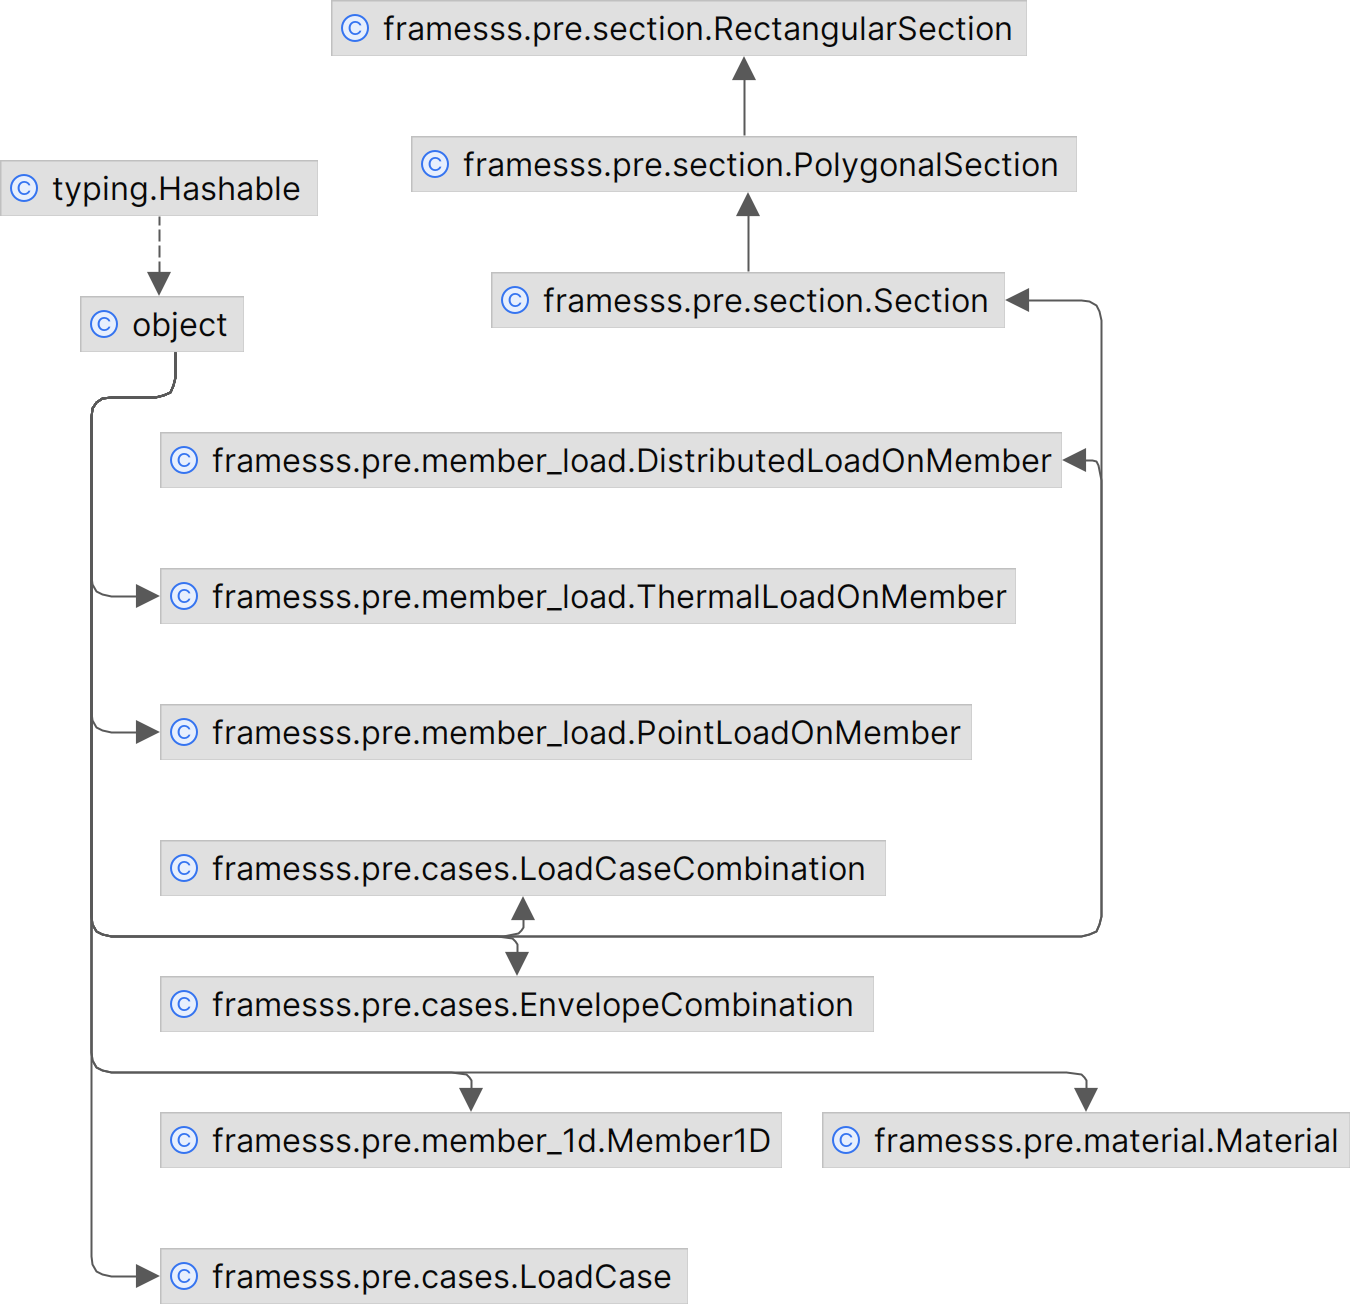
\includegraphics{assets/figures/framesss/uml/pre.png}
    \caption{Diagram modulu \texttt{pre}}
    \label{fig:modul_pre}
\end{figure}

%%%%%%%%%%%%%%%%%%%%%%%%%%%%%%%%%%%%%%%% FEA %%%%%%%%%%%%%%%%%%%%%%%%%%%%%%%%%%%%%%%%%%%%%%%

\subsubsection*{Modul \texttt{fea}}
Na obr. \ref{fig:modul_fea} je diagram zobrazující hierarchii tříd v~modulu 
\href{https://danberanek.github.io/framesss/gen/framesss.fea.html}{\texttt{fea}}, který je srdcem knihovny framesss. Klíčovou třídou je
\href{https://danberanek.github.io/framesss/gen/framesss.fea.models.model.Model.html#framesss.fea.models.model.Model}{\texttt{Model}}, která je zodpovědná za přidávání prvků (uzly, prvky, zatěžovací stavy, zatížení atd.) a drží v~sobě všechny instance, které se následně předávají do řešiče (solveru). Pod ní jsou specifické modely, jako
\href{https://danberanek.github.io/framesss/gen/framesss.fea.models.frame_xz.FrameXZModel.html#framesss.fea.models.frame_xz.FrameXZModel}{\texttt{FrameXZModel}}. Modul také obsahuje třídy pro definici elementů
\href{https://danberanek.github.io/framesss/gen/framesss.fea.element_1d.Element1D.html#framesss.fea.element_1d.Element1D}{\texttt{Element1D}}
 a uzlů
 \href{https://danberanek.github.io/framesss/gen/framesss.fea.node.Node.html#framesss.fea.node.Node}{ \texttt{Node}}. Pro zatížení elementů zde máme abstraktní třídu 
 \href{https://danberanek.github.io/framesss/gen/framesss.fea.boundary_conditions.element_load.ElementLoad.html#framesss.fea.boundary_conditions.element_load.ElementLoad}{\texttt{ElementLoad}}, ze které vychází třída pro zatížení spojitým zatížením
 \href{https://danberanek.github.io/framesss/gen/framesss.fea.boundary_conditions.element_load.DistributedLoad.html}{\texttt{DistributedLoad}}
 a třída pro zatížení teplotou
 \href{https://danberanek.github.io/framesss/gen/framesss.fea.boundary_conditions.element_load.ThermalLoad.html}{\texttt{ThermalLoad}}, dále je zde třída pro uzlové zatížení
 \href{https://danberanek.github.io/framesss/gen/framesss.fea.boundary_conditions.nodal_load.NodalLoad.html}{\texttt{NodalLoad}}, a pro předepsané přemístění podpor
\href{https://danberanek.github.io/framesss/gen/framesss.fea.boundary_conditions.prescribed_displacement.PrescribedDisplacement.html#framesss.fea.boundary_conditions.prescribed_displacement.PrescribedDisplacement}{ \texttt{PrescribedDisplacement}}.
 Modul také zahrnuje třídy pro specifikování dimenze problému, které vychází z~abstraktní třídy
 \href{https://danberanek.github.io/framesss/gen/framesss.fea.analysis.analysis.Analysis.html#framesss.fea.analysis.analysis.Analysis}{\texttt{Analysis}}
 a její konkrétní implementace pro různé typy konstrukcí, např.
 \href{https://danberanek.github.io/framesss/gen/framesss.fea.analysis.frame_xz_analysis.FrameXZAnalysis.html#framesss.fea.analysis.frame_xz_analysis.FrameXZAnalysis}{\texttt{FrameXZAnalysis}}.

\begin{figure}[H]
    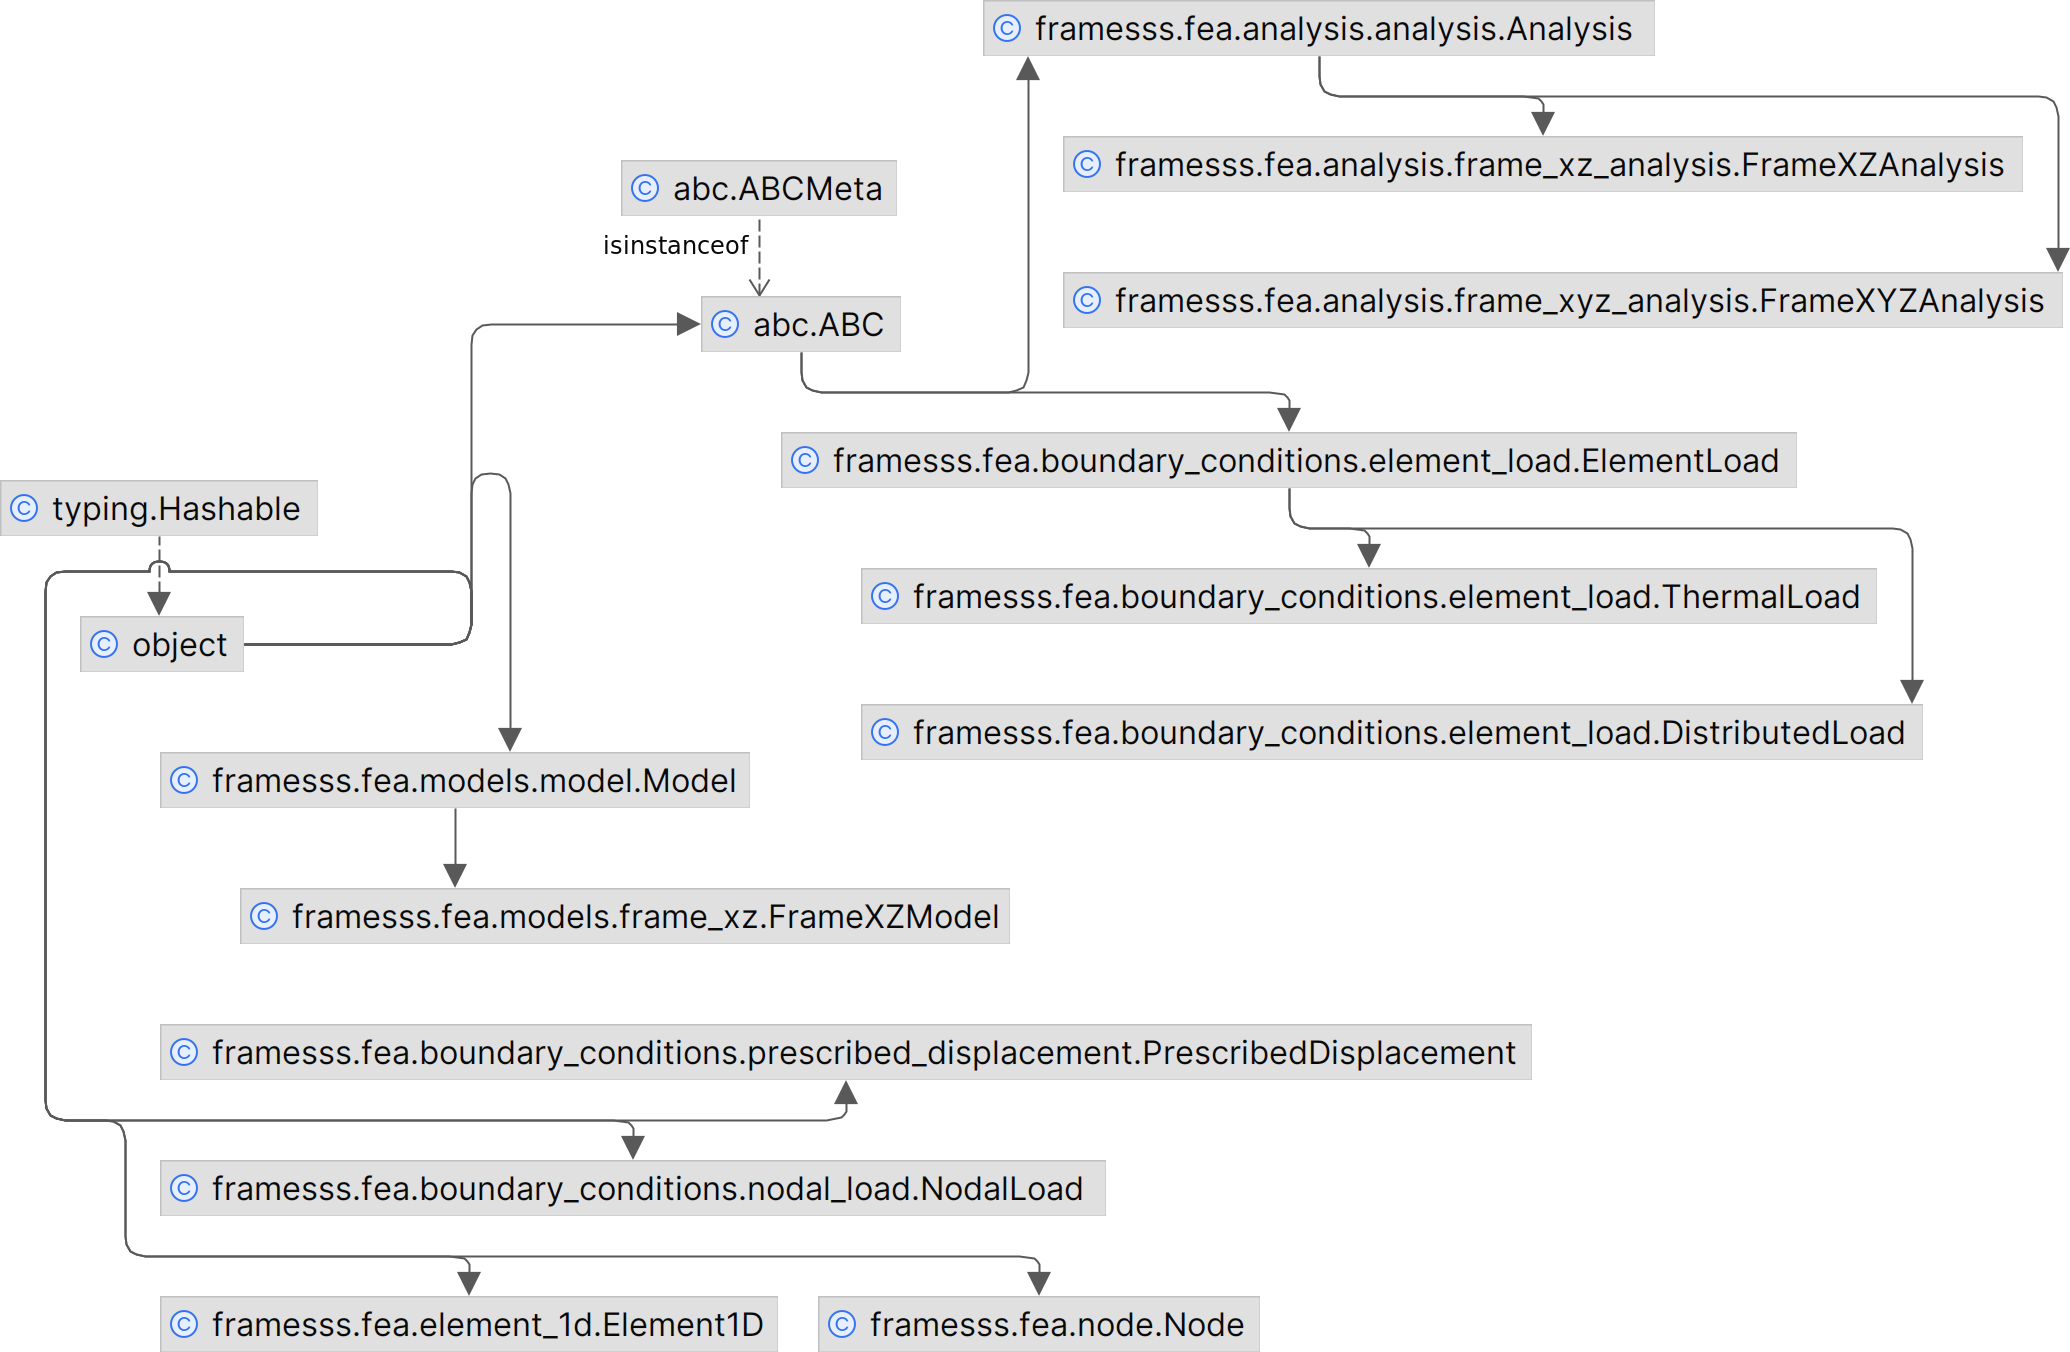
\includegraphics{assets/figures/framesss/uml/fea.png}
    \caption{Diagram modulu \texttt{fea}}
    \label{fig:modul_fea}
\end{figure}

\subsubsection*{Modul \texttt{solvers}}
Modul obsahuje řešiče používané pro výpočty v~modulu
\href{https://danberanek.github.io/framesss/gen/framesss.fea.html}{\texttt{fea}}. Na  obr. \ref{fig:modul_solvers} je znázorněný diagram hierarchie tříd v~modulu
\href{https://danberanek.github.io/framesss/gen/framesss.solvers.html}{\texttt{solvers}}. Základem této hierarchie je třída \texttt{abc.ABC}, což je základní abstraktní třída v~Pythonu. Na jejím základě je definována třída
\href{https://danberanek.github.io/framesss/gen/framesss.solvers.solver.Solver.html}{\texttt{Solver}}, která slouží jako základ pro konkrétní implementace řešičů. Jediným implementovaným řešičem je v~současné době třída
\href{https://danberanek.github.io/framesss/gen/framesss.solvers.linear_static.LinearStaticSolver.html}{\texttt{LinearStaticSolver}}, která implementuje lineární statické výpočty.

\begin{figure}[H]
    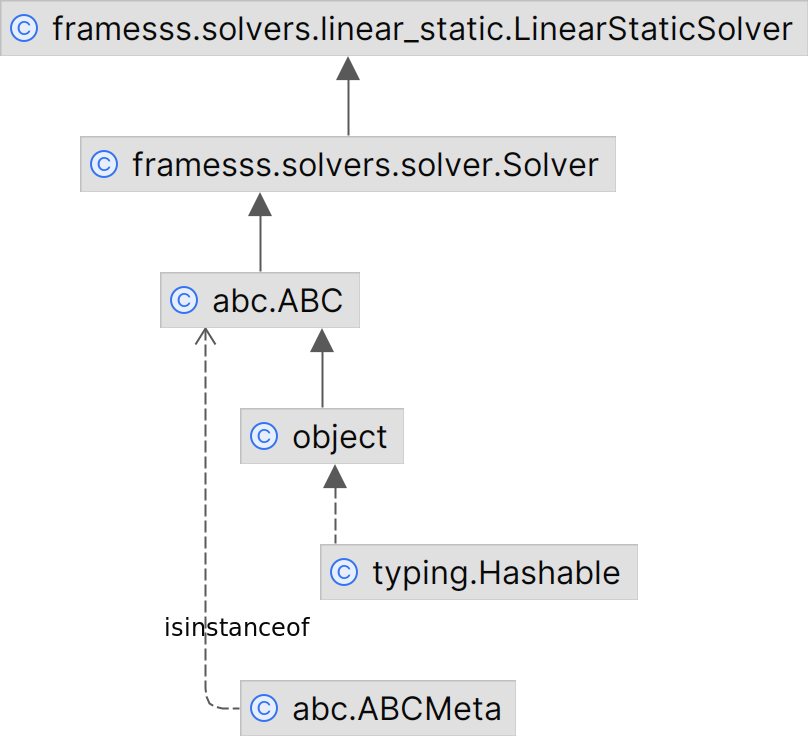
\includegraphics{assets/figures/framesss/uml/solvers.png}
    \caption{Diagram modulu \texttt{solvers}}
    \label{fig:modul_solvers}
\end{figure}

\subsubsection*{Modul \texttt{post}}
Zpracovává výsledky, jako jsou posuny a vnitřní síly, které jsou získány z~výpočtu provedených modulem \href{https://danberanek.github.io/framesss/gen/framesss.fea.html}{\texttt{fea}}. Modul nezahrnuje vizualizaci, ale umožňuje uživatelům extrahovat a prohlížet vypočítané hodnoty, které mohou být dále použity.
Diagram na obr. \ref{fig:modul_post} ukazuje hierarchii tříd v~modulu \href{https://danberanek.github.io/framesss/gen/framesss.post.html}{\texttt{post}}, který je zodpovědný za zpracování výsledků. Třída 
\href{https://danberanek.github.io/framesss/gen/framesss.post.member_1d_results.Member1DResults.html#framesss.post.member_1d_results.Member1DResults}{\texttt{Member1DResults}} zpracovává výsledky pro jednotlivé prutové prvky, třída
\href{https://danberanek.github.io/framesss/gen/framesss.post.node_results.NodeResults.html}{\texttt{NodeResults}} zpracovává výsledky pro jednotlivé uzly konstrukce.
\begin{figure}[H]
    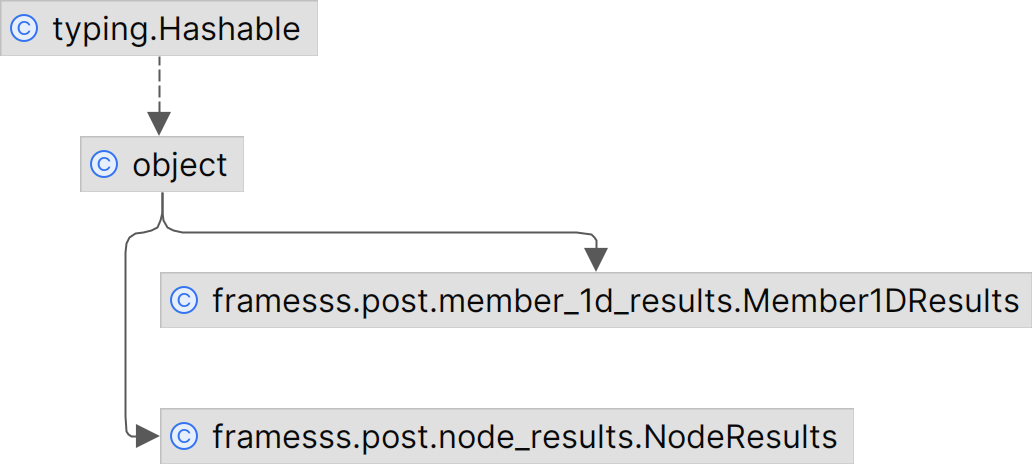
\includegraphics{assets/figures/framesss/uml/post.png}
    \caption{Diagram modulu \texttt{post}}
    \label{fig:modul_post}
\end{figure}

\subsection{Předpoklady}

V této sekci jsou uvedeny základní předpoklady, které byly přijaty při vývoji knihovny \texttt{framesss},
\begin{itemize}
    \item konstrukce je umístěna v pravotočivé souřadné soustavě,
    \item pro kladný směr pootočení platí pravidlo pravé ruky\footnote{Palec natočíme ve směru kladné části osy a zahnuté prsty pravé ruky značí kladný směr otáčení.},
    \item výpočet probíhá podle teorie malých deformací,
    \item materiál je uvažován jako pružný, platí Hookův zákon.
\end{itemize}

Tyto předpoklady umožňují uplatnění principu superpozice.

\subsubsection*{Předpoklady pro model v rovině XZ}

\begin{itemize}
    \item zatížení působí pouze v rovině \gls{X}\gls{Z}, která je zároveň rovinou symetrie,
    \item každý uzel má přiřazené tři stupně volnosti, posun ve směru globální osy \gls{X}, pootočení okolo globální osy \gls{Y} a posun ve směru globální osy \gls{Z}. Kladný směr je naznačený na \autoref{fig:global_dofs},    
    \begin{figure}[H]
        \begin{tikzpicture}[>={Stealth[inset=0pt,length=8pt,angle'=28,round]}]
    \draw[->] (0, 0) -- (2,0) node[above] {\gls{X}, +\gls{u_i}};
    \draw[->] (0, 0) -- (0,-2) node[right] {\gls{Z}, +\gls{w_i}};
    \draw[->,domain=180:450] plot ({cos(\x)}, {sin(\x)}) node[above right] {+\gls{phi_i}};
\end{tikzpicture}
        \caption{Stupně volnosti v globálním systému}
        \label{fig:global_dofs}
    \end{figure}

    \item stupně volnosti a jejich kódová čísla\footnote{Indexování v jazyce Python začíná od $0$, což znamená, že první stupeň volnosti má přiřazené kódové číslo $0$, druhý prvek má kódové číslo $1$ atd.} v lokálním systému prutového prvku jsou označena na \autoref{fig:dof_numbering},
    
    \begin{figure}[H]
        \begin{tikzpicture}[>={Stealth[inset=0pt,length=8pt,angle'=28,round]}]
    \draw[->] (-0.5, -0.5) -- (1,-0.5) node[above] {\gls{X}};
    \draw[->] (-0.5, -0.5) -- (-0.5,1) node[left] {\gls{Z}};

    \draw[dotted,->] (2, 2) -- (9,3.75) node[above] {\gls{x}};
    \draw[dotted,->] (2, 2) -- (1.5,4) node[above] {\gls{z}};
    \point{a}{2}{2};
    \point{b}{6}{3};

    \beam{1}{a}{b}[1][1]

    \draw[fill=white] (2,2) circle (.25cm) node[text=black] {$i$};
    \draw[fill=white] (6,3) circle (.25cm) node[text=black] {$j$};

    \draw[<-] ($(2,2)!0.35cm!(1,1.75)$) -- (0.5, 1.625) node[text=ctublue,above] {0};
    \draw[<-] ($(2,2)!0.35cm!(2.5,0)$) -- (2.375, 0.5) node[text=ctublue,right] {2};
    \draw[->,domain=330:60] plot ({2 + cos(\x)}, {2 + sin(\x)}) node[text=ctublue, above right] {1};

    \draw[->] ($(6,3)!0.35cm!(10,4)$) -- (7.5, 3.375) node[text=ctublue,above] {3};
    \draw[<-] ($(6,3)!0.35cm!(6.5,1)$) -- (6.375, 1.5) node[text=ctublue,right] {5};
    \draw[->,domain=330:60] plot ({6 + cos(\x)}, {3 + sin(\x)}) node[text=ctublue, above right] {4};

\end{tikzpicture}
        \caption{Stupně volnosti v lokálním systému prvku}
        \label{fig:dof_numbering}
    \end{figure}

    \item vnitřní síly v jakémkoliv průřezu prvku jsou: normálová síla \gls{axial_force}, posouvající síla \gls{shear_force} a ohybový moment \gls{bending_moment}. Kladná orientace vnitřních sil je naznačená na \autoref{fig:positive_internal_forces}.
    \begin{figure}[H]
        \begin{tikzpicture}
    \point{a}{0}{0}
    \point{b}{1.5}{0}

    \beam{1}{a}{b}[1][1]

    \load{1}{b}[90][1][-1.1]
    \point{n1}{2.6}{0}
    \notation{1}{n1}{\gls{axial_force}}[above left]

    \load{1}{b}[180][1][-1.1]
    \point{v1}{1.5}{-1.1}
    \notation{1}{v1}{\gls{shear_force}}[above right]

    \load{3}{b}[225]
    \point{m1}{1.4}{0.3}
    \notation{1}{m1}{\gls{bending_moment}}[above left]

    \point{c}{4.5}{0}
    \point{d}{6}{0}
    \beam{1}{c}{d}[1][1]

    \load{1}{c}[0][1][-1.1]
    \point{n2}{3.4}{0}
    \notation{1}{n2}{\gls{axial_force}}[above right]

    \load{1}{c}[270][1][-1.1]
    \point{v2}{4.5}{1}
    \notation{1}{v2}{\gls{shear_force}}[below right]

    \load{2}{c}[135]
    \point{m2}{4.5}{-0.4}
    \notation{1}{m2}{\gls{bending_moment}}[below]

\end{tikzpicture}
        \caption{Kladná orientace vnitřních sil}
        \label{fig:positive_internal_forces}
    \end{figure}
\end{itemize}


\subsection{Algoritmizace}

V~této sekci je představen algoritmus, který je jádrem metody konečných prvků implementované v~knihovně framesss. Tento algoritmus systematicky zpracovává model od jeho diskretizace až po výpočet odezvy konstrukce na zatížení jednotlivými zatěžovacími stavy a jejich kombinacemi.

\begin{algorithm}[H]
    \caption{Proces výpočtu modelu}
    \DontPrintSemicolon  % Don't print semicolons
    
    \SetKwFunction{FMain}{solve()}
    \SetKwProg{Fn}{Metoda}{:}{}
    \Fn{\FMain}{
        Diskretizace prutů na jednotlivé elementy\;
        Očíslování stupňů volnosti\;
        Lokalizace globální matice tuhosti\;
        \For{každý zatěžovací stav}{
            Inicializace vektoru koncových posunů\;
            Lokalizace předepsaných deformací\;
            Inicializace vektoru zatížení\;
            Lokalizace sil v~uzlech\;
            Lokalizace koncových sil na prvcích\; 
            Výpočet vektoru neznámých koncových posunů\;
            Výpočet reakcí\;
            Výpočet koeficientů vnitřních sil\;
            Výpočet extrémů vnitřních sil\;
            Uložení vypočítaných hodnot\;
        }
        \For{každá kombinace zatížení}{
            Inicializace výsledků\;
            \For{každý zatěžovací stav v~kombinaci}{
                Přičtení hodnot k~výsledkům\;
            }
            Uložení výsledků\;
        }
        \For{každá obálka}{
            Inicializace\;
            Určení extrémních hodnot v~každé kombinaci\;
            Uložení hodnot\;
        }
        \Return{}
    }
    
\end{algorithm}

\subsection{Řídké matice}

V rámci knihovny \texttt{framesss} je zásadní efektivní manipulace s řídkými maticemi, které se často vyskytují v důsledku velkého množství nulových prvků v maticích tuhosti. Pro ukládání a zpracování těchto matic využívá \texttt{framesss} knihovnu SciPy \cite{scipy}, specificky její modul pro řídké matice.

\subsubsection{Formáty ukládání řídkých matic}

V rámci knihovny SciPy jsou k dispozici různé formáty pro ukládání řídkých matic, z nichž každý je optimalizován pro specifické typy operací.

\begin{itemize}
    \item \textbf{CSR (Compressed Sparse Row)}: Ukládá data kompresí řádkových indexů. Tento formát je efektivní pro řádkové operace.
    \item \textbf{CSC (Compressed Sparse Column)}: Podobné jako CSR, ale komprimuje sloupcové indexy. Je efektivní pro sloupcové operace.
    \item \textbf{BSR (Block Sparse Row)}: Velmi podobný formátu CSR. Je vhodný pro řídké matice s hustými submaticemi.
    \item \textbf{COO (COOrdinate format)}: Ukládá seznam trojic (řádkový index, sloupcový index a hodnotu), což umožňuje efektivní postupné sestavování řídkých matic.
    \item \textbf{DIA (DIAgonal storage)}: Ukládá hodnoty na diagonálách v samostatných polích a jejich offset od diagonály, což je užitečné pro matice s dominantními diagonálami.
    \item \textbf{DOK (Dictionary Of Keys)}: Ukládá prvky matice ve slovníku, kde klíče jsou dvojice (řádek, sloupec).
    \item \textbf{LIL (LIst of Lists)}: Ukládá matice pomocí dvou seznamů, jeden pro řádky, ve kterých jsou ukládány sloupcové indexy, a druhý pro hodnoty.
\end{itemize}


\subsubsection{Využití ve \texttt{framesss}}

Proces vytváření a manipulace s řídkými maticemi v knihovně \texttt{framesss} zahrnuje několik klíčových kroků, které využívají různé formáty matic pro optimalizaci různých fází výpočtu:

\begin{enumerate}
    \item \textbf{Vytvoření matice jako COO}: Ve fázi lokalizace je globální matice tuhosti vytvářena jako COO, což je formát efektivní pro konstrukci řídkých matic
    
    \item \textbf{Převod do LIL}: Po sestavení základní struktury matice je převedena do formátu LIL pro rychlé řezání (slicing), indexování a manipulaci. LIL umožňuje efektivní změny řádků a sloupců matice, což je vyžadováno během dělení soustavy rovnic na dvě soustavy rovnic.
    
    \item \textbf{Převod do CSR}: Konečný převod matice do formátu CSR je proveden pro rychlé aritmetické operace, které jsou nezbytné pro  řešení systému rovnic. CSR formát je vysoce optimalizovaný pro rychlé maticové operace.
\end{enumerate}

Každý z těchto formátů má specifické výhody pro různé typy operací a jejich výběr je motivován potřebou maximalizovat výpočetní efektivitu a minimalizovat dobu provádění v různých fázích výpočetního procesu. Použití COO pro počáteční sestavení, LIL pro manipulaci s řádky a sloupci a CSR pro finální výpočty umožňuje dosáhnout optimálního výkonu.


\subsection{Testování}

Pro zajištění spolehlivosti a přesnosti knihovny \texttt{framesss} byla implementována řada automatizovaných testů. Automatizované testování umožňuje včasné odhalení a opravu chyb, což přispívá k celkové stabilitě a kvalitě knihovny.

Testování knihovny \texttt{framesss} probíhá v různých verzích Pythonu (3.9, 3.10, 3.11, 3.12), aby byla odhalena případná kolize v závislostech mezi verzemi. Lokálně jsou testy spouštěny pomocí nástroje \texttt{nox} \cite{nox}, který vytváří virtuální prostředí, instaluje potřebné knihovny a spouští všechny testy, včetně validačních, \texttt{pre-commit} \cite{precommit} a \texttt{mypy} \cite{mypy} testů.

\subsubsection*{Unit testy}
Unit test je základní typ testu používaný v softwarovém vývoji, jehož cílem je ověřit správnou funkci jednotlivých částí kódu. Unit testy se zaměřují na testování nejmenších, izolovaných částí aplikace, jako jsou jednotlivé funkce nebo metody tříd. Hlavní charakteristiky unit testů jsou
\begin{itemize}
    \item \textbf{Izolace}: Testy jsou navrženy tak, aby byly nezávislé na ostatních částech kódu. Každý test kontroluje pouze jednu konkrétní část funkčnosti.
    \item \textbf{Automatizace}: Testy jsou spouštěny automaticky, což umožňuje rychlou a efektivní kontrolu správnosti
    \item \textbf{Opakovatelnost}: Testy mohou být opakovaně spouštěny při každé změně kódu, což zajišťuje, že nové změny neovlivní existující funkčnost.
\end{itemize}

\subsubsection*{Validační testy}
Kromě unit testů se správnost knihovny testuje na jednoduchých konstrukcích (prostý nosník, šikmé nosníky, konzoly, oboustranně vetknutý nosník apd.), kde je známé analytické řešení.

Pro validační testy byly použity následující zdroje:
\begin{itemize}
    \item \textit{DESIGN AID No. 6 — BEAM DESIGN FORMULAR WITH SHEAR AND MOMENT DIAGRAMS} od American Wood Council \cite{design_aid},
    \item \textit{Sbírka příkladů stavební mechaniky: princip virtuálních sil, silová metoda, deformační metoda} od Jíra, A. a kol. \cite{sbirka_prikladu}.
\end{itemize}

\subsubsection*{Kontinuální integrace a spuštění testů na GitHubu}
Kromě lokálního testování je nezbytné zajistit, aby všechny změny v kódu byly automaticky testovány i při jejich nahrání do centrálního repozitáře. Tento proces, známý jako kontinuální integrace (Continuous Integration, CI), je implementován pomocí GitHub Actions.

Při každém pushnutí změn do GitHub repozitáře se automaticky spustí CI pipeline, která zahrnuje následující kroky:
\begin{itemize}
    \item \textbf{Instalace závislostí}: Nezbytné knihovny a závislosti jsou nainstalovány podle specifikací v konfiguračním souboru.
    \item \textbf{Statická analýza kódu}: Kód je zkontrolován nástrojem mypy \cite{mypy}, který provádí statickou typovou kontrolu, aby se zajistila konzistence typů a odhalily potenciální typové chyby.
    \item \textbf{Spuštění unit testů}: Pomocí nástroje pytest \cite{pytest} se spustí všechny unit testy a validační testy, aby se ověřila funkčnost všech částí kódu.
\end{itemize}

Jednou z výhod používání GitHub Actions je možnost testovat kód na různých operačních systémech, knihovna \texttt{framesss} je testován na následujících platformách
\begin{itemize}
    \item \textbf{Windows},
    \item \textbf{Linux},
    \item \textbf{MacOS}.
\end{itemize}

\subsection{Příklad}

Následující příklad je převzat ze \textit{Sbírky příkladů stavební mechaniky} \cite[Příklad 5.2]{sbirka_prikladu}.

\begin{figure}[H]
    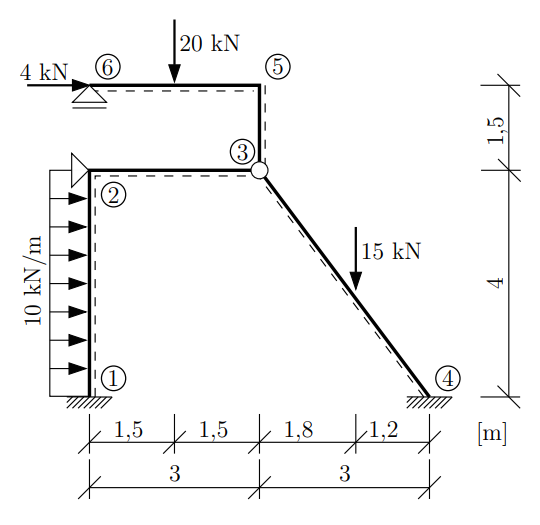
\includegraphics[height=7cm]{assets/figures/framesss/example_snk.png}
    \caption[Statické schéma konstrukce]{Statické schéma konstrukce, převzato z \cite[Příklad 5.2]{sbirka_prikladu}}
    \label{fig:framesss_example}
\end{figure}

Všechny pruty mají Youngův modul pružnosti $\gls{E} = \SI{30}{\GPa}$, moment setrvačnosti k ose, kolem které jsou pruty namáhané ohybem $\gls{I_y} = \SI{1e-3}{\unit{\metre\tothe{4}}}$ a plochu $\gls{A}= \SI{4e-3}{{\metre\tothe{2}}}$.

Na příkladu bude ilustrováno použití knihovny \texttt{framesss} v prostředí JupyterLab.

V prvním kroku je nutné importovat knihovny, se kterými budeme pracovat.

\begin{tcolorbox}[breakable, size=fbox, boxrule=1pt, pad at break*=1mm,colback=cellbackground, colframe=cellborder]
    \prompt{In}{incolor}{1}{\boxspacing}
    \begin{Verbatim}[commandchars=\\\{\}]
    \PY{k+kn}{import} \PY{n+nn}{numpy} \PY{k}{as} \PY{n+nn}{np}
    
    \PY{k+kn}{from} \PY{n+nn}{tabulate} \PY{k+kn}{import} \PY{n}{tabulate}
    
    \PY{k+kn}{from} \PY{n+nn}{framesss}\PY{n+nn}{.}\PY{n+nn}{fea}\PY{n+nn}{.}\PY{n+nn}{models}\PY{n+nn}{.}\PY{n+nn}{frame\PYZus{}xz} \PY{k+kn}{import} \PY{n}{FrameXZModel}
    \PY{k+kn}{from} \PY{n+nn}{framesss}\PY{n+nn}{.}\PY{n+nn}{pre}\PY{n+nn}{.}\PY{n+nn}{material} \PY{k+kn}{import} \PY{n}{Material}
    \PY{k+kn}{from} \PY{n+nn}{framesss}\PY{n+nn}{.}\PY{n+nn}{pre}\PY{n+nn}{.}\PY{n+nn}{section} \PY{k+kn}{import} \PY{n}{Section}
    \PY{k+kn}{from} \PY{n+nn}{framesss}\PY{n+nn}{.}\PY{n+nn}{solvers}\PY{n+nn}{.}\PY{n+nn}{linear\PYZus{}static} \PY{k+kn}{import} \PY{n}{LinearStaticSolver}
    \end{Verbatim}
\end{tcolorbox}

Začneme definicí materiálu, knihovna nepracuje s převody jednotek, musíme být konzistentní. Zvolíme systém jednotek $\text{kN, kPa a m}$. Poissonův součinitel \gls{nu}, teplotní součinitel roztažnosti, ani objemovou hmotnost materiálu bychom nemuseli definovat, protože mají výchozí hodnoty, ale uvádíme je zde pro přehlednost.
\begin{tcolorbox}[breakable, size=fbox, boxrule=1pt, pad at break*=1mm,colback=cellbackground, colframe=cellborder]
    \prompt{In}{incolor}{2}{\boxspacing}
    \begin{Verbatim}[commandchars=\\\{\}]
    \PY{n}{material} \PY{o}{=} \PY{n}{Material}\PY{p}{(}
        \PY{n}{label}\PY{o}{=}\PY{l+s+s2}{\PYZdq{}}\PY{l+s+s2}{foo}\PY{l+s+s2}{\PYZdq{}}\PY{p}{,}
        \PY{n}{elastic\PYZus{}modulus}\PY{o}{=}\PY{l+m+mf}{30.e6}\PY{p}{,}
        \PY{n}{poissons\PYZus{}ratio}\PY{o}{=}\PY{l+m+mf}{0.2}\PY{p}{,}
        \PY{n}{thermal\PYZus{}expansion\PYZus{}coefficient}\PY{o}{=}\PY{l+m+mf}{1.0e\PYZhy{}3}\PY{p}{,}
        \PY{n}{density}\PY{o}{=}\PY{l+m+mf}{0.0}\PY{p}{,}
    \PY{p}{)}
    \end{Verbatim}
\end{tcolorbox}

Jako další definujeme průřez prvku pomocí třídy \texttt{Section}, proměnná \texttt{area\_x} slouží pro výpočet normálové tuhosti, \texttt{area\_y} a \texttt{area\_z} se ve výpočtu použijí pouze v případě, že prutový prvek, kterému tento průřez přiřadíme bude typu \texttt{'timoshenko'}. Plocha zadaná těmto atributům má odpovídat hodnotě $k \gls{A}$, kde k je korekční součinitel rozložení smykového napětí. Pro získání správného výsledku je dále potřeba přiřadit správnou hodnotu momentu setrvačnosti \gls{I_y} do atributu \texttt{inertia\_y} a přiřadit materiál definovaný v předchozí buňce, ostatní hodnoty při tomto výpočtu nehrají roli, uvádíme je pouze pro přehlednost.
\begin{tcolorbox}[breakable, size=fbox, boxrule=1pt, pad at break*=1mm,colback=cellbackground, colframe=cellborder]
    \prompt{In}{incolor}{3}{\boxspacing}
    \begin{Verbatim}[commandchars=\\\{\}]
    \PY{n}{section} \PY{o}{=} \PY{n}{Section}\PY{p}{(}
        \PY{n}{label}\PY{o}{=}\PY{l+s+s2}{\PYZdq{}}\PY{l+s+s2}{bar}\PY{l+s+s2}{\PYZdq{}}\PY{p}{,}
        \PY{n}{area\PYZus{}x}\PY{o}{=}\PY{l+m+mf}{4.0e\PYZhy{}3}\PY{p}{,}
        \PY{n}{area\PYZus{}y}\PY{o}{=}\PY{l+m+mf}{1.0}\PY{p}{,}
        \PY{n}{area\PYZus{}z}\PY{o}{=}\PY{l+m+mf}{1.0}\PY{p}{,}
        \PY{n}{inertia\PYZus{}x}\PY{o}{=}\PY{l+m+mf}{1.0}\PY{p}{,}
        \PY{n}{inertia\PYZus{}y}\PY{o}{=}\PY{l+m+mf}{1.0e\PYZhy{}3}\PY{p}{,}
        \PY{n}{inertia\PYZus{}z}\PY{o}{=}\PY{l+m+mf}{1.0}\PY{p}{,}
        \PY{n}{height\PYZus{}z}\PY{o}{=}\PY{l+m+mf}{1.0}\PY{p}{,}
        \PY{n}{height\PYZus{}y}\PY{o}{=}\PY{l+m+mf}{1.0}\PY{p}{,}
        \PY{n}{material}\PY{o}{=}\PY{n}{material}
    \PY{p}{)}
    \end{Verbatim}
\end{tcolorbox}

V dalším kroku vytvoříme instanci modelu \texttt{FrameXZModel}. Pomocí metod této třídy budeme modelovat celou konstrukci i se zatížením.
\begin{tcolorbox}[breakable, size=fbox, boxrule=1pt, pad at break*=1mm,colback=cellbackground, colframe=cellborder]
    \prompt{In}{incolor}{4}{\boxspacing}
    \begin{Verbatim}[commandchars=\\\{\}]
    \PY{n}{model} \PY{o}{=} \PY{n}{FrameXZModel}\PY{p}{(}\PY{p}{)}
    \end{Verbatim}
\end{tcolorbox}

Pomocí metody \texttt{add\_node()} definujeme uzly konstrukce. Atributy, které musíme zadat jsou označení uzlu \texttt{label} a souřadnice uzlu \texttt{coords} ve formátu [\gls{X}, \gls{Y}, \gls{Z}]. Nepovinným atributem metody je \texttt{fixity}, kterou definujeme okrajové podmínky pro každý stupeň volnosti v uzlu, zadáváme je pomocí stringů \texttt{'fixed'} nebo \texttt{'free'} a řadíme je v pořadí [\gls{u_i}[ ], \gls{v_i}[ ], \gls{w_i}[ ], \gls{phi_i}[\gls{x}], \gls{phi_i}[\gls{y}], \gls{phi_i}[\gls{z}]].
\begin{tcolorbox}[breakable, size=fbox, boxrule=1pt, pad at break*=1mm,colback=cellbackground, colframe=cellborder]
    \prompt{In}{incolor}{5}{\boxspacing}
    \begin{Verbatim}[commandchars=\\\{\}]
    \PY{n}{N1} \PY{o}{=} \PY{n}{model}\PY{o}{.}\PY{n}{add\PYZus{}node}\PY{p}{(}
        \PY{n}{label}\PY{o}{=}\PY{l+s+s2}{\PYZdq{}}\PY{l+s+s2}{N1}\PY{l+s+s2}{\PYZdq{}}\PY{p}{,}
        \PY{n}{coords}\PY{o}{=}\PY{p}{[}\PY{l+m+mf}{0.0}\PY{p}{,} \PY{l+m+mf}{0.0}\PY{p}{,} \PY{l+m+mf}{0.0}\PY{p}{]}\PY{p}{,}
        \PY{n}{fixity}\PY{o}{=}\PY{p}{[}\PY{l+s+s1}{\PYZsq{}}\PY{l+s+s1}{fixed}\PY{l+s+s1}{\PYZsq{}}\PY{p}{,} \PY{l+s+s1}{\PYZsq{}}\PY{l+s+s1}{free}\PY{l+s+s1}{\PYZsq{}}\PY{p}{,} \PY{l+s+s1}{\PYZsq{}}\PY{l+s+s1}{fixed}\PY{l+s+s1}{\PYZsq{}}\PY{p}{,} \PY{l+s+s1}{\PYZsq{}}\PY{l+s+s1}{free}\PY{l+s+s1}{\PYZsq{}}\PY{p}{,} \PY{l+s+s1}{\PYZsq{}}\PY{l+s+s1}{fixed}\PY{l+s+s1}{\PYZsq{}}\PY{p}{,} \PY{l+s+s1}{\PYZsq{}}\PY{l+s+s1}{free}\PY{l+s+s1}{\PYZsq{}}\PY{p}{]}\PY{p}{,}
    \PY{p}{)}
    
    \PY{n}{N2} \PY{o}{=} \PY{n}{model}\PY{o}{.}\PY{n}{add\PYZus{}node}\PY{p}{(}
        \PY{n}{label}\PY{o}{=}\PY{l+s+s2}{\PYZdq{}}\PY{l+s+s2}{N2}\PY{l+s+s2}{\PYZdq{}}\PY{p}{,}
        \PY{n}{coords}\PY{o}{=}\PY{p}{[}\PY{l+m+mf}{0.0}\PY{p}{,} \PY{l+m+mf}{0.0}\PY{p}{,} \PY{l+m+mf}{4.0}\PY{p}{]}\PY{p}{,}
        \PY{n}{fixity}\PY{o}{=}\PY{p}{[}\PY{l+s+s2}{\PYZdq{}}\PY{l+s+s2}{fixed}\PY{l+s+s2}{\PYZdq{}}\PY{p}{,} \PY{l+s+s2}{\PYZdq{}}\PY{l+s+s2}{free}\PY{l+s+s2}{\PYZdq{}}\PY{p}{,} \PY{l+s+s2}{\PYZdq{}}\PY{l+s+s2}{fixed}\PY{l+s+s2}{\PYZdq{}}\PY{p}{,} \PY{l+s+s2}{\PYZdq{}}\PY{l+s+s2}{free}\PY{l+s+s2}{\PYZdq{}}\PY{p}{,} \PY{l+s+s2}{\PYZdq{}}\PY{l+s+s2}{free}\PY{l+s+s2}{\PYZdq{}}\PY{p}{,} \PY{l+s+s2}{\PYZdq{}}\PY{l+s+s2}{free}\PY{l+s+s2}{\PYZdq{}}\PY{p}{]}\PY{p}{,}
    \PY{p}{)}
    
    \PY{n}{N3} \PY{o}{=} \PY{n}{model}\PY{o}{.}\PY{n}{add\PYZus{}node}\PY{p}{(}
        \PY{n}{label}\PY{o}{=}\PY{l+s+s2}{\PYZdq{}}\PY{l+s+s2}{N3}\PY{l+s+s2}{\PYZdq{}}\PY{p}{,}
        \PY{n}{coords}\PY{o}{=}\PY{p}{[}\PY{l+m+mf}{3.0}\PY{p}{,} \PY{l+m+mf}{0.0}\PY{p}{,} \PY{l+m+mf}{4.0}\PY{p}{]}\PY{p}{,}
    \PY{p}{)}
    
    \PY{n}{N4} \PY{o}{=} \PY{n}{model}\PY{o}{.}\PY{n}{add\PYZus{}node}\PY{p}{(}
        \PY{n}{label}\PY{o}{=}\PY{l+s+s2}{\PYZdq{}}\PY{l+s+s2}{N4}\PY{l+s+s2}{\PYZdq{}}\PY{p}{,}
        \PY{n}{coords}\PY{o}{=}\PY{p}{[}\PY{l+m+mf}{6.0}\PY{p}{,} \PY{l+m+mf}{0.0}\PY{p}{,} \PY{l+m+mf}{0.0}\PY{p}{]}\PY{p}{,}
        \PY{n}{fixity}\PY{o}{=}\PY{p}{[}\PY{l+s+s2}{\PYZdq{}}\PY{l+s+s2}{fixed}\PY{l+s+s2}{\PYZdq{}}\PY{p}{,} \PY{l+s+s2}{\PYZdq{}}\PY{l+s+s2}{free}\PY{l+s+s2}{\PYZdq{}}\PY{p}{,} \PY{l+s+s2}{\PYZdq{}}\PY{l+s+s2}{fixed}\PY{l+s+s2}{\PYZdq{}}\PY{p}{,} \PY{l+s+s2}{\PYZdq{}}\PY{l+s+s2}{free}\PY{l+s+s2}{\PYZdq{}}\PY{p}{,} \PY{l+s+s2}{\PYZdq{}}\PY{l+s+s2}{fixed}\PY{l+s+s2}{\PYZdq{}}\PY{p}{,} \PY{l+s+s2}{\PYZdq{}}\PY{l+s+s2}{free}\PY{l+s+s2}{\PYZdq{}}\PY{p}{]}
    \PY{p}{)}
    
    \PY{n}{N5} \PY{o}{=} \PY{n}{model}\PY{o}{.}\PY{n}{add\PYZus{}node}\PY{p}{(}
        \PY{n}{label}\PY{o}{=}\PY{l+s+s2}{\PYZdq{}}\PY{l+s+s2}{N5}\PY{l+s+s2}{\PYZdq{}}\PY{p}{,}
        \PY{n}{coords}\PY{o}{=}\PY{p}{[}\PY{l+m+mf}{3.0}\PY{p}{,} \PY{l+m+mf}{0.0}\PY{p}{,} \PY{l+m+mf}{5.5}\PY{p}{]}\PY{p}{,}
    \PY{p}{)}
    
    \PY{n}{N6} \PY{o}{=} \PY{n}{model}\PY{o}{.}\PY{n}{add\PYZus{}node}\PY{p}{(}
        \PY{n}{label}\PY{o}{=}\PY{l+s+s2}{\PYZdq{}}\PY{l+s+s2}{N6}\PY{l+s+s2}{\PYZdq{}}\PY{p}{,}
        \PY{n}{coords}\PY{o}{=}\PY{p}{[}\PY{l+m+mf}{0.0}\PY{p}{,} \PY{l+m+mf}{0.0}\PY{p}{,} \PY{l+m+mf}{5.5}\PY{p}{]}\PY{p}{,}
        \PY{n}{fixity}\PY{o}{=}\PY{p}{[}\PY{l+s+s1}{\PYZsq{}}\PY{l+s+s1}{free}\PY{l+s+s1}{\PYZsq{}}\PY{p}{,} \PY{l+s+s1}{\PYZsq{}}\PY{l+s+s1}{free}\PY{l+s+s1}{\PYZsq{}}\PY{p}{,} \PY{l+s+s1}{\PYZsq{}}\PY{l+s+s1}{fixed}\PY{l+s+s1}{\PYZsq{}}\PY{p}{,} \PY{l+s+s1}{\PYZsq{}}\PY{l+s+s1}{free}\PY{l+s+s1}{\PYZsq{}}\PY{p}{,} \PY{l+s+s1}{\PYZsq{}}\PY{l+s+s1}{free}\PY{l+s+s1}{\PYZsq{}}\PY{p}{,} \PY{l+s+s1}{\PYZsq{}}\PY{l+s+s1}{free}\PY{l+s+s1}{\PYZsq{}}\PY{p}{]}
    \PY{p}{)}
    \end{Verbatim}
\end{tcolorbox}

Pomocí metody \texttt{add\_member()} přidáme jednotlivé pruty. Atributy jsou označení \texttt{label}, typ použitého elementu \texttt{element\_type}, který může být buď \texttt{'navier'} pro prut bez vlivu smyku nebo \texttt{'timoshenko'} pro prut s vlivem smyku. Dále zadáme počáteční a koncový uzel, průřez prvku a můžeme zadat nepovinný atribut \texttt{hinges}, který udává, zda je v odpovídajícím uzlu prut připojen kloubově nebo pevně.
\begin{tcolorbox}[breakable, size=fbox, boxrule=1pt, pad at break*=1mm,colback=cellbackground, colframe=cellborder]
    \prompt{In}{incolor}{6}{\boxspacing}
    \begin{Verbatim}[commandchars=\\\{\}]
    \PY{n}{B12} \PY{o}{=} \PY{n}{model}\PY{o}{.}\PY{n}{add\PYZus{}member}\PY{p}{(}
        \PY{n}{label}\PY{o}{=}\PY{l+s+s2}{\PYZdq{}}\PY{l+s+s2}{1\PYZhy{}2}\PY{l+s+s2}{\PYZdq{}}\PY{p}{,}
        \PY{n}{element\PYZus{}type}\PY{o}{=}\PY{l+s+s2}{\PYZdq{}}\PY{l+s+s2}{navier}\PY{l+s+s2}{\PYZdq{}}\PY{p}{,}
        \PY{n}{nodes}\PY{o}{=}\PY{p}{[}\PY{n}{N1}\PY{p}{,} \PY{n}{N2}\PY{p}{]}\PY{p}{,}
        \PY{n}{section}\PY{o}{=}\PY{n}{section}\PY{p}{,}
    \PY{p}{)}
    
    \PY{n}{B23} \PY{o}{=} \PY{n}{model}\PY{o}{.}\PY{n}{add\PYZus{}member}\PY{p}{(}
        \PY{n}{label}\PY{o}{=}\PY{l+s+s2}{\PYZdq{}}\PY{l+s+s2}{2\PYZhy{}3}\PY{l+s+s2}{\PYZdq{}}\PY{p}{,}
        \PY{n}{element\PYZus{}type}\PY{o}{=}\PY{l+s+s2}{\PYZdq{}}\PY{l+s+s2}{navier}\PY{l+s+s2}{\PYZdq{}}\PY{p}{,}
        \PY{n}{nodes}\PY{o}{=}\PY{p}{[}\PY{n}{N2}\PY{p}{,} \PY{n}{N3}\PY{p}{]}\PY{p}{,}
        \PY{n}{section}\PY{o}{=}\PY{n}{section}\PY{p}{,}
        \PY{n}{hinges}\PY{o}{=}\PY{p}{[}\PY{l+s+s2}{\PYZdq{}}\PY{l+s+s2}{fixed}\PY{l+s+s2}{\PYZdq{}}\PY{p}{,} \PY{l+s+s2}{\PYZdq{}}\PY{l+s+s2}{hinged}\PY{l+s+s2}{\PYZdq{}}\PY{p}{]}\PY{p}{,}
    \PY{p}{)}
    
    \PY{n}{B34} \PY{o}{=} \PY{n}{model}\PY{o}{.}\PY{n}{add\PYZus{}member}\PY{p}{(}
        \PY{n}{label}\PY{o}{=}\PY{l+s+s2}{\PYZdq{}}\PY{l+s+s2}{3\PYZhy{}4}\PY{l+s+s2}{\PYZdq{}}\PY{p}{,}
        \PY{n}{element\PYZus{}type}\PY{o}{=}\PY{l+s+s2}{\PYZdq{}}\PY{l+s+s2}{navier}\PY{l+s+s2}{\PYZdq{}}\PY{p}{,}
        \PY{n}{nodes}\PY{o}{=}\PY{p}{[}\PY{n}{N3}\PY{p}{,} \PY{n}{N4}\PY{p}{]}\PY{p}{,}
        \PY{n}{section}\PY{o}{=}\PY{n}{section}\PY{p}{,}
        \PY{n}{hinges}\PY{o}{=}\PY{p}{[}\PY{l+s+s2}{\PYZdq{}}\PY{l+s+s2}{hinged}\PY{l+s+s2}{\PYZdq{}}\PY{p}{,} \PY{l+s+s2}{\PYZdq{}}\PY{l+s+s2}{fixed}\PY{l+s+s2}{\PYZdq{}}\PY{p}{]}\PY{p}{,}
    \PY{p}{)}
    
    \PY{n}{B35} \PY{o}{=} \PY{n}{model}\PY{o}{.}\PY{n}{add\PYZus{}member}\PY{p}{(}
        \PY{n}{label}\PY{o}{=}\PY{l+s+s2}{\PYZdq{}}\PY{l+s+s2}{3\PYZhy{}5}\PY{l+s+s2}{\PYZdq{}}\PY{p}{,}
        \PY{n}{element\PYZus{}type}\PY{o}{=}\PY{l+s+s2}{\PYZdq{}}\PY{l+s+s2}{navier}\PY{l+s+s2}{\PYZdq{}}\PY{p}{,}
        \PY{n}{nodes}\PY{o}{=}\PY{p}{[}\PY{n}{N3}\PY{p}{,} \PY{n}{N5}\PY{p}{]}\PY{p}{,}
        \PY{n}{section}\PY{o}{=}\PY{n}{section}\PY{p}{,}
        \PY{n}{hinges}\PY{o}{=}\PY{p}{[}\PY{l+s+s2}{\PYZdq{}}\PY{l+s+s2}{hinged}\PY{l+s+s2}{\PYZdq{}}\PY{p}{,} \PY{l+s+s2}{\PYZdq{}}\PY{l+s+s2}{fixed}\PY{l+s+s2}{\PYZdq{}}\PY{p}{]}\PY{p}{,}
    \PY{p}{)}
    
    \PY{n}{B65} \PY{o}{=} \PY{n}{model}\PY{o}{.}\PY{n}{add\PYZus{}member}\PY{p}{(}
        \PY{n}{label}\PY{o}{=}\PY{l+s+s2}{\PYZdq{}}\PY{l+s+s2}{6\PYZhy{}5}\PY{l+s+s2}{\PYZdq{}}\PY{p}{,}
        \PY{n}{element\PYZus{}type}\PY{o}{=}\PY{l+s+s2}{\PYZdq{}}\PY{l+s+s2}{navier}\PY{l+s+s2}{\PYZdq{}}\PY{p}{,}
        \PY{n}{nodes}\PY{o}{=}\PY{p}{[}\PY{n}{N6}\PY{p}{,} \PY{n}{N5}\PY{p}{]}\PY{p}{,}
        \PY{n}{section}\PY{o}{=}\PY{n}{section}\PY{p}{,}
    \PY{p}{)}
    \end{Verbatim}
\end{tcolorbox}

V dalším kroku definujeme zatížení. Zatěžovací stav do modelu přidáme pomocí metody \texttt{add\_load\_case()}. Jednotlivé síly a spojitá zatížení přidáváme přímo na dříve definované instance prutů a uzlů pomocí metod \texttt{add\_distributed\_load()} a \texttt{add\_point\_load()} pro pruty, případně \texttt{add\_nodal\_load()} pro uzly. Výchozí směr zatížení je v globálním souřadném systému. Polohu spojitého zatížení zadáváme pomocí atributů \texttt{x\_start} a \texttt{x\_end}, hodnoty zadáváme hodnotou na začátku a na konci intervalu pro směry \gls{x}, \gls{y} a \gls{z}. Tímto přístupem je možné modelovat lichoběžníkové zatížení kdekoliv na nosníku. Pomocí metody \texttt{add\_point\_load()} lze přidat osamělou sílu nebo moment, hodnoty musí být v pořadí $[F_{\gls{x}}, F_{\gls{y}}, F_{\gls{z}}, M_{\gls{x}}, M_{\gls{y}}, M_{\gls{z}}]$.
\begin{tcolorbox}[breakable, size=fbox, boxrule=1pt, pad at break*=1mm,colback=cellbackground, colframe=cellborder]
    \prompt{In}{incolor}{7}{\boxspacing}
    \begin{Verbatim}[commandchars=\\\{\}]
        \PY{n}{LC1} \PY{o}{=} \PY{n}{model}\PY{o}{.}\PY{n}{add\PYZus{}load\PYZus{}case}\PY{p}{(}
            \PY{n}{label}\PY{o}{=}\PY{l+s+s1}{\PYZsq{}}\PY{l+s+s1}{LC1}\PY{l+s+s1}{\PYZsq{}}
        \PY{p}{)}
        
        \PY{n}{B12}\PY{o}{.}\PY{n}{add\PYZus{}distributed\PYZus{}load}\PY{p}{(}
            \PY{n}{load\PYZus{}components}\PY{o}{=}\PY{p}{[}\PY{l+m+mf}{10.}\PY{p}{,} \PY{l+m+mf}{0.}\PY{p}{,} \PY{l+m+mf}{0.}\PY{p}{,} \PY{l+m+mf}{10.}\PY{p}{,} \PY{l+m+mf}{0.}\PY{p}{,} \PY{l+m+mf}{0.}\PY{p}{]}\PY{p}{,}
            \PY{n}{load\PYZus{}case}\PY{o}{=}\PY{n}{LC1}\PY{p}{,}
            \PY{n}{x\PYZus{}start}\PY{o}{=}\PY{l+m+mf}{0.0}\PY{p}{,}
            \PY{n}{x\PYZus{}end}\PY{o}{=}\PY{l+m+mf}{1.0}\PY{p}{,}
            \PY{n}{coordinate\PYZus{}system}\PY{o}{=}\PY{l+s+s2}{\PYZdq{}}\PY{l+s+s2}{global}\PY{l+s+s2}{\PYZdq{}}\PY{p}{,}
            \PY{n}{location}\PY{o}{=}\PY{l+s+s2}{\PYZdq{}}\PY{l+s+s2}{length}\PY{l+s+s2}{\PYZdq{}}\PY{p}{,}
            \PY{n}{coordinate\PYZus{}definition}\PY{o}{=}\PY{l+s+s2}{\PYZdq{}}\PY{l+s+s2}{relative}\PY{l+s+s2}{\PYZdq{}}\PY{p}{,}
        \PY{p}{)}
        
        \PY{n}{B34}\PY{o}{.}\PY{n}{add\PYZus{}point\PYZus{}load}\PY{p}{(}
            \PY{n}{load\PYZus{}components}\PY{o}{=}\PY{p}{[}\PY{l+m+mf}{0.}\PY{p}{,} \PY{l+m+mf}{0.}\PY{p}{,} \PY{o}{\PYZhy{}}\PY{l+m+mf}{15.}\PY{p}{,} \PY{l+m+mf}{0.}\PY{p}{,} \PY{l+m+mf}{0.}\PY{p}{,} \PY{l+m+mf}{0.}\PY{p}{]}\PY{p}{,}
            \PY{n}{load\PYZus{}case}\PY{o}{=}\PY{n}{LC1}\PY{p}{,}
            \PY{n}{x}\PY{o}{=}\PY{l+m+mf}{1.8}\PY{o}{/}\PY{l+m+mi}{3}\PY{p}{,}
            \PY{n}{coordinate\PYZus{}system}\PY{o}{=}\PY{l+s+s2}{\PYZdq{}}\PY{l+s+s2}{global}\PY{l+s+s2}{\PYZdq{}}\PY{p}{,}
            \PY{n}{coordinate\PYZus{}definition}\PY{o}{=}\PY{l+s+s2}{\PYZdq{}}\PY{l+s+s2}{relative}\PY{l+s+s2}{\PYZdq{}}\PY{p}{,}
        \PY{p}{)}
        
        \PY{n}{B65}\PY{o}{.}\PY{n}{add\PYZus{}point\PYZus{}load}\PY{p}{(}
            \PY{n}{load\PYZus{}components}\PY{o}{=}\PY{p}{[}\PY{l+m+mf}{0.}\PY{p}{,} \PY{l+m+mf}{0.}\PY{p}{,} \PY{o}{\PYZhy{}}\PY{l+m+mf}{20.}\PY{p}{,} \PY{l+m+mf}{0.}\PY{p}{,} \PY{l+m+mf}{0.}\PY{p}{,} \PY{l+m+mf}{0.}\PY{p}{]}\PY{p}{,}
            \PY{n}{load\PYZus{}case}\PY{o}{=}\PY{n}{LC1}\PY{p}{,}
            \PY{n}{x}\PY{o}{=}\PY{l+m+mf}{0.5}\PY{p}{,}
        \PY{p}{)}
        
        \PY{n}{N6}\PY{o}{.}\PY{n}{add\PYZus{}nodal\PYZus{}load}\PY{p}{(}
            \PY{n}{load\PYZus{}components}\PY{o}{=}\PY{p}{[}\PY{l+m+mf}{4.}\PY{p}{,} \PY{l+m+mf}{0.}\PY{p}{,} \PY{l+m+mf}{0.}\PY{p}{,} \PY{l+m+mf}{0.}\PY{p}{,} \PY{l+m+mf}{0.}\PY{p}{,} \PY{l+m+mf}{0.}\PY{p}{]}\PY{p}{,}
            \PY{n}{load\PYZus{}case}\PY{o}{=}\PY{n}{LC1}\PY{p}{,}
        \PY{p}{)}
    \end{Verbatim}
\end{tcolorbox}

To samé zatížení přidáme do modelu ještě jednou, tentokrát však každé zatížení přiřadíme jinému zatěžovacímu stavu, poté z jednotlivých stavů vytvoříme novou kombinaci zatížení. Hodnoty zatížení vydělíme součiniteli \texttt{LC<i>\_factor} a při vytváření nové kombinace tento součinitel použijeme jako součinitel kombinace.
\begin{tcolorbox}[breakable, size=fbox, boxrule=1pt, pad at break*=1mm,colback=cellbackground, colframe=cellborder]
    \prompt{In}{incolor}{8}{\boxspacing}
    \begin{Verbatim}[commandchars=\\\{\}]
    \PY{n}{LC2\PYZus{}factor} \PY{o}{=} \PY{l+m+mi}{2}
    \PY{n}{LC3\PYZus{}factor} \PY{o}{=} \PY{l+m+mi}{18}
    \PY{n}{LC4\PYZus{}factor} \PY{o}{=} \PY{l+m+mf}{5.5}
    \PY{n}{LC5\PYZus{}factor} \PY{o}{=} \PY{o}{\PYZhy{}}\PY{l+m+mi}{12}
    
    \PY{n}{LC2} \PY{o}{=} \PY{n}{model}\PY{o}{.}\PY{n}{add\PYZus{}load\PYZus{}case}\PY{p}{(}
        \PY{n}{label}\PY{o}{=}\PY{l+s+s2}{\PYZdq{}}\PY{l+s+s2}{LC2}\PY{l+s+s2}{\PYZdq{}}
    \PY{p}{)}
    \PY{n}{B12}\PY{o}{.}\PY{n}{add\PYZus{}distributed\PYZus{}load}\PY{p}{(}
        \PY{n}{load\PYZus{}components}\PY{o}{=}\PY{n}{np}\PY{o}{.}\PY{n}{array}\PY{p}{(}
            \PY{p}{[}\PY{l+m+mf}{10.}\PY{p}{,} \PY{l+m+mf}{0.}\PY{p}{,} \PY{l+m+mf}{0.}\PY{p}{,} \PY{l+m+mf}{10.}\PY{p}{,} \PY{l+m+mf}{0.}\PY{p}{,} \PY{l+m+mf}{0.}\PY{p}{]}
        \PY{p}{)} \PY{o}{/} \PY{n}{LC2\PYZus{}factor}\PY{p}{,}
        \PY{n}{load\PYZus{}case}\PY{o}{=}\PY{n}{LC2}\PY{p}{,}
    \PY{p}{)}
    
    \PY{n}{LC3} \PY{o}{=} \PY{n}{model}\PY{o}{.}\PY{n}{add\PYZus{}load\PYZus{}case}\PY{p}{(}
        \PY{n}{label}\PY{o}{=}\PY{l+s+s2}{\PYZdq{}}\PY{l+s+s2}{LC3}\PY{l+s+s2}{\PYZdq{}}
    \PY{p}{)}
    \PY{n}{B34}\PY{o}{.}\PY{n}{add\PYZus{}point\PYZus{}load}\PY{p}{(}
        \PY{n}{load\PYZus{}components}\PY{o}{=}\PY{n}{np}\PY{o}{.}\PY{n}{array}\PY{p}{(}
            \PY{p}{[}\PY{l+m+mf}{0.}\PY{p}{,} \PY{l+m+mf}{0.}\PY{p}{,} \PY{o}{\PYZhy{}}\PY{l+m+mf}{15.}\PY{p}{,} \PY{l+m+mf}{0.}\PY{p}{,} \PY{l+m+mf}{0.}\PY{p}{,} \PY{l+m+mf}{0.}\PY{p}{]}
        \PY{p}{)} \PY{o}{/} \PY{n}{LC3\PYZus{}factor}\PY{p}{,}
        \PY{n}{load\PYZus{}case}\PY{o}{=}\PY{n}{LC3}\PY{p}{,}
        \PY{n}{x}\PY{o}{=}\PY{l+m+mf}{1.8}\PY{o}{/}\PY{l+m+mi}{3}\PY{p}{,}
    \PY{p}{)}
    
    \PY{n}{LC4} \PY{o}{=}  \PY{n}{model}\PY{o}{.}\PY{n}{add\PYZus{}load\PYZus{}case}\PY{p}{(}
        \PY{n}{label}\PY{o}{=}\PY{l+s+s2}{\PYZdq{}}\PY{l+s+s2}{LC4}\PY{l+s+s2}{\PYZdq{}}
    \PY{p}{)}
    \PY{n}{B65}\PY{o}{.}\PY{n}{add\PYZus{}point\PYZus{}load}\PY{p}{(}
        \PY{n}{load\PYZus{}components}\PY{o}{=}\PY{n}{np}\PY{o}{.}\PY{n}{array}\PY{p}{(}
            \PY{p}{[}\PY{l+m+mf}{0.}\PY{p}{,} \PY{l+m+mf}{0.}\PY{p}{,} \PY{o}{\PYZhy{}}\PY{l+m+mf}{20.}\PY{p}{,} \PY{l+m+mf}{0.}\PY{p}{,} \PY{l+m+mf}{0.}\PY{p}{,} \PY{l+m+mf}{0.}\PY{p}{]}
        \PY{p}{)} \PY{o}{/} \PY{n}{LC4\PYZus{}factor}\PY{p}{,}
        \PY{n}{load\PYZus{}case}\PY{o}{=}\PY{n}{LC4}\PY{p}{,}
        \PY{n}{x}\PY{o}{=}\PY{l+m+mf}{0.5}\PY{p}{,}
    \PY{p}{)}
    
    \PY{n}{LC5} \PY{o}{=} \PY{n}{model}\PY{o}{.}\PY{n}{add\PYZus{}load\PYZus{}case}\PY{p}{(}
        \PY{n}{label}\PY{o}{=}\PY{l+s+s2}{\PYZdq{}}\PY{l+s+s2}{LC5}\PY{l+s+s2}{\PYZdq{}}
    \PY{p}{)}
    \PY{n}{N6}\PY{o}{.}\PY{n}{add\PYZus{}nodal\PYZus{}load}\PY{p}{(}
        \PY{n}{load\PYZus{}components}\PY{o}{=}\PY{n}{np}\PY{o}{.}\PY{n}{array}\PY{p}{(}
            \PY{p}{[}\PY{l+m+mf}{4.}\PY{p}{,} \PY{l+m+mf}{0.}\PY{p}{,} \PY{l+m+mf}{0.}\PY{p}{,} \PY{l+m+mf}{0.}\PY{p}{,} \PY{l+m+mf}{0.}\PY{p}{,} \PY{l+m+mf}{0.}\PY{p}{]}
        \PY{p}{)} \PY{o}{/} \PY{n}{LC5\PYZus{}factor}\PY{p}{,}
        \PY{n}{load\PYZus{}case}\PY{o}{=}\PY{n}{LC5}\PY{p}{,}
    \PY{p}{)}
    
    \PY{n}{CO1} \PY{o}{=} \PY{n}{model}\PY{o}{.}\PY{n}{add\PYZus{}load\PYZus{}case\PYZus{}combination}\PY{p}{(}
        \PY{n}{label}\PY{o}{=}\PY{l+s+s2}{\PYZdq{}}\PY{l+s+s2}{CO1}\PY{l+s+s2}{\PYZdq{}}\PY{p}{,}
        \PY{n}{combination}\PY{o}{=}\PY{p}{\PYZob{}}
            \PY{n}{LC2}\PY{p}{:} \PY{n}{LC2\PYZus{}factor}\PY{p}{,}
            \PY{n}{LC3}\PY{p}{:} \PY{n}{LC3\PYZus{}factor}\PY{p}{,}
            \PY{n}{LC4}\PY{p}{:} \PY{n}{LC4\PYZus{}factor}\PY{p}{,}
            \PY{n}{LC5}\PY{p}{:} \PY{n}{LC5\PYZus{}factor}\PY{p}{,}
        \PY{p}{\PYZcb{}}
    \PY{p}{)}
    \end{Verbatim}
\end{tcolorbox}

Vytvoříme instanci řešiče a propojíme ho s instancí \texttt{model}.
\begin{tcolorbox}[breakable, size=fbox, boxrule=1pt, pad at break*=1mm,colback=cellbackground, colframe=cellborder]
    \prompt{In}{incolor}{9}{\boxspacing}
    \begin{Verbatim}[commandchars=\\\{\}]
    \PY{n}{solver} \PY{o}{=} \PY{n}{LinearStaticSolver}\PY{p}{(}
        \PY{n}{model}\PY{o}{=}\PY{n}{model}
    \PY{p}{)}
    \end{Verbatim}
\end{tcolorbox}

Výpočet provedeme pomocí metody \texttt{solve()}.
\begin{tcolorbox}[breakable, size=fbox, boxrule=1pt, pad at break*=1mm,colback=cellbackground, colframe=cellborder]
    \prompt{In}{incolor}{10}{\boxspacing}
    \begin{Verbatim}[commandchars=\\\{\}]
    \PY{n}{solver}\PY{o}{.}\PY{n}{solve}\PY{p}{(}\PY{p}{)}
    \end{Verbatim}
\end{tcolorbox}

Výsledky jsou uložené v instancích tříd \texttt{Node} a \texttt{Member1D} v objektu \texttt{results}. Pomocí metody {get()}, dostaneme výsledky pro zatěžovací stavy nebo kombinace. Hodnoty nakonec vypíšeme do tabulky. V tabulce si můžeme všimnout, že program vytvořil vlastní uzly v místech působících osamělých sil.
\begin{tcolorbox}[breakable, size=fbox, boxrule=1pt, pad at break*=1mm,colback=cellbackground, colframe=cellborder]
    \prompt{In}{incolor}{11}{\boxspacing}
    \begin{Verbatim}[commandchars=\\\{\}]
    \PY{n}{displacements}\PY{o}{=} \PY{p}{[}\PY{p}{]}
    \PY{n}{reactions} \PY{o}{=} \PY{p}{[}\PY{p}{]}
    \PY{k}{for} \PY{n}{node} \PY{o+ow}{in} \PY{n}{model}\PY{o}{.}\PY{n}{nodes}\PY{p}{:}
        \PY{k}{for} \PY{n}{case} \PY{o+ow}{in} \PY{p}{[}\PY{n}{LC1}\PY{p}{,} \PY{n}{CO1}\PY{p}{]}\PY{p}{:}
            \PY{n}{displacements}\PY{o}{.}\PY{n}{append}\PY{p}{(}\PY{p}{[}
                \PY{k}{case}\PY{o}{.}\PY{n}{label}\PY{p}{,}
                \PY{n}{node}\PY{o}{.}\PY{n}{label}\PY{p}{,}
                \PY{n}{node}\PY{o}{.}\PY{n}{results}\PY{o}{.}\PY{n}{translation\PYZus{}x}\PY{o}{.}\PY{n}{get}\PY{p}{(}\PY{n}{case}\PY{p}{)}\PY{p}{,}
                \PY{n}{node}\PY{o}{.}\PY{n}{results}\PY{o}{.}\PY{n}{translation\PYZus{}z}\PY{o}{.}\PY{n}{get}\PY{p}{(}\PY{n}{case}\PY{p}{)}\PY{p}{,}
                \PY{n}{node}\PY{o}{.}\PY{n}{results}\PY{o}{.}\PY{n}{rotation\PYZus{}y}\PY{o}{.}\PY{n}{get}\PY{p}{(}\PY{n}{case}\PY{p}{)}\PY{p}{,}
            \PY{p}{]}\PY{p}{)}
            \PY{n}{r\PYZus{}x} \PY{o}{=} \PY{n}{node}\PY{o}{.}\PY{n}{results}\PY{o}{.}\PY{n}{reaction\PYZus{}force\PYZus{}x}\PY{o}{.}\PY{n}{get}\PY{p}{(}\PY{n}{case}\PY{p}{)}
            \PY{n}{r\PYZus{}z} \PY{o}{=} \PY{n}{node}\PY{o}{.}\PY{n}{results}\PY{o}{.}\PY{n}{reaction\PYZus{}force\PYZus{}z}\PY{o}{.}\PY{n}{get}\PY{p}{(}\PY{n}{case}\PY{p}{)}
            \PY{n}{r\PYZus{}my} \PY{o}{=} \PY{n}{node}\PY{o}{.}\PY{n}{results}\PY{o}{.}\PY{n}{reaction\PYZus{}moment\PYZus{}y}\PY{o}{.}\PY{n}{get}\PY{p}{(}\PY{n}{case}\PY{p}{)}
    
            \PY{k}{if} \PY{n}{r\PYZus{}x} \PY{o+ow}{or} \PY{n}{r\PYZus{}z} \PY{o+ow}{or} \PY{n}{r\PYZus{}my}\PY{p}{:}
                \PY{n}{reactions}\PY{o}{.}\PY{n}{append}\PY{p}{(}\PY{p}{[}
                    \PY{k}{case}\PY{o}{.}\PY{n}{label}\PY{p}{,}
                    \PY{n}{node}\PY{o}{.}\PY{n}{label}\PY{p}{,}
                    \PY{n}{r\PYZus{}x}\PY{p}{,}
                    \PY{n}{r\PYZus{}z}\PY{p}{,}
                    \PY{n}{r\PYZus{}my}
                \PY{p}{]}\PY{p}{)}
            
        \PY{n}{displacements}\PY{o}{.}\PY{n}{append}\PY{p}{(}\PY{p}{[}\PY{k+kc}{None}\PY{p}{]} \PY{o}{*} \PY{l+m+mi}{5}\PY{p}{)}
        \PY{k}{if} \PY{n}{r\PYZus{}x} \PY{o+ow}{or} \PY{n}{r\PYZus{}z} \PY{o+ow}{or} \PY{n}{r\PYZus{}my}\PY{p}{:}
            \PY{n}{reactions}\PY{o}{.}\PY{n}{append}\PY{p}{(}\PY{p}{[}\PY{k+kc}{None}\PY{p}{]} \PY{o}{*} \PY{l+m+mi}{5}\PY{p}{)}
    
    \PY{n+nb}{print}\PY{p}{(}\PY{n}{tabulate}\PY{p}{(}
        \PY{n}{displacements}\PY{p}{,}
        \PY{n}{headers}\PY{o}{=}\PY{p}{[}\PY{l+s+s2}{\PYZdq{}}\PY{l+s+s2}{case}\PY{l+s+s2}{\PYZdq{}}\PY{p}{,} \PY{l+s+s2}{\PYZdq{}}\PY{l+s+s2}{node}\PY{l+s+s2}{\PYZdq{}}\PY{p}{,} \PY{l+s+s2}{\PYZdq{}}\PY{l+s+s2}{u\PYZus{}x}\PY{l+s+s2}{\PYZdq{}}\PY{p}{,} \PY{l+s+s2}{\PYZdq{}}\PY{l+s+s2}{u\PYZus{}z}\PY{l+s+s2}{\PYZdq{}}\PY{p}{,} \PY{l+s+s2}{\PYZdq{}}\PY{l+s+s2}{phi\PYZus{}y}\PY{l+s+s2}{\PYZdq{}}\PY{p}{]}\PY{p}{,}
        \PY{n}{tablefmt}\PY{o}{=}\PY{l+s+s2}{\PYZdq{}}\PY{l+s+s2}{rst}\PY{l+s+s2}{\PYZdq{}}\PY{p}{,}
        \PY{n}{floatfmt}\PY{o}{=}\PY{l+s+s2}{\PYZdq{}}\PY{l+s+s2}{.3e}\PY{l+s+s2}{\PYZdq{}}
    \PY{p}{)}\PY{p}{)}
    \PY{n+nb}{print}\PY{p}{(}\PY{n}{tabulate}\PY{p}{(}
        \PY{n}{reactions}\PY{p}{,}
        \PY{n}{headers}\PY{o}{=}\PY{p}{[}\PY{l+s+s2}{\PYZdq{}}\PY{l+s+s2}{case}\PY{l+s+s2}{\PYZdq{}}\PY{p}{,} \PY{l+s+s2}{\PYZdq{}}\PY{l+s+s2}{node}\PY{l+s+s2}{\PYZdq{}}\PY{p}{,} \PY{l+s+s2}{\PYZdq{}}\PY{l+s+s2}{R\PYZus{}x}\PY{l+s+s2}{\PYZdq{}}\PY{p}{,} \PY{l+s+s2}{\PYZdq{}}\PY{l+s+s2}{R\PYZus{}z}\PY{l+s+s2}{\PYZdq{}}\PY{p}{,} \PY{l+s+s2}{\PYZdq{}}\PY{l+s+s2}{R\PYZus{}My}\PY{l+s+s2}{\PYZdq{}}\PY{p}{]}\PY{p}{,}
        \PY{n}{tablefmt}\PY{o}{=}\PY{l+s+s2}{\PYZdq{}}\PY{l+s+s2}{rst}\PY{l+s+s2}{\PYZdq{}}\PY{p}{,}
        \PY{n}{floatfmt}\PY{o}{=}\PY{l+s+s2}{\PYZdq{}}\PY{l+s+s2}{.3f}\PY{l+s+s2}{\PYZdq{}}
    \PY{p}{)}\PY{p}{)}
    \end{Verbatim}
    \end{tcolorbox}
    
\begin{Verbatim}[commandchars=\\\{\}]
    ======  ======  ==========  ==========  ==========
    case    node           u\_x         u\_z       phi\_y
    ======  ======  ==========  ==========  ==========
    LC1     N1       0.000e+00   0.000e+00   0.000e+00
    CO1     N1       0.000e+00   0.000e+00   0.000e+00

    LC1     N2       0.000e+00   0.000e+00  -6.942e-05
    CO1     N2       0.000e+00   0.000e+00  -6.942e-05
    
    LC1     N3      -9.902e-05  -9.168e-04   0.000e+00
    CO1     N3      -9.902e-05  -9.168e-04   0.000e+00

    LC1     N4       0.000e+00   0.000e+00   0.000e+00
    CO1     N4       0.000e+00   0.000e+00   0.000e+00
    
    LC1     N5       3.219e-04  -1.067e-03   1.806e-04
    CO1     N5       3.219e-04  -1.067e-03   1.806e-04
    
    LC1     N6       4.219e-04   0.000e+00   6.306e-04
    CO1     N6       4.219e-04   0.000e+00   6.306e-04
        
    LC1     3-4(1)  -7.831e-05  -5.457e-04  -2.216e-04
    CO1     3-4(1)  -7.831e-05  -5.457e-04  -2.216e-04
    
    LC1     6-5(1)   3.719e-04  -7.959e-04   3.306e-04
    CO1     6-5(1)   3.719e-04  -7.959e-04   3.306e-04

    ======  ======  ==========  ==========  ==========

    ======  ======  =======  ======  =======
    case    node        R\_x     R\_z     R\_My
    ======  ======  =======  ======  =======
    LC1     N1      -20.781   0.000  -14.375
    CO1     N1      -20.781   0.000  -14.375
     
    LC1     N2      -15.258   3.750
    CO1     N2      -15.258   3.750

    LC1     N4       -7.961  23.250   10.905
    CO1     N4       -7.961  23.250   10.905

    LC1     N6                8.000
    CO1     N6                8.000
    ======  ======  =======  ======  =======
        \end{Verbatim}
    

\begin{figure}[H]
    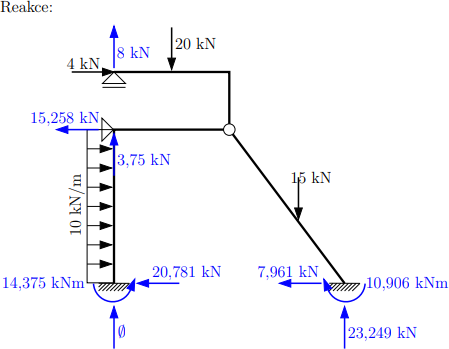
\includegraphics{assets/figures/framesss/example_reactions.png}
    \caption[Reakce v podporách]{Reakce v podporách, převzato z \cite[Příklad 5.2]{sbirka_prikladu}}
    \label{fig:framesss_example_reactions}
\end{figure}

    Stejně jako v případu uzlů, výsledky se ukládají do objektu \texttt{results}, do tabulky vypíšeme extrémy vnitřních sil pro jednotlivé prvky.
        \begin{tcolorbox}[breakable, size=fbox, boxrule=1pt, pad at break*=1mm,colback=cellbackground, colframe=cellborder]
    \prompt{In}{incolor}{12}{\boxspacing}
    \begin{Verbatim}[commandchars=\\\{\}]
    \PY{n}{headers} \PY{o}{=} \PY{p}{[}\PY{l+s+s2}{\PYZdq{}}\PY{l+s+s2}{case}\PY{l+s+s2}{\PYZdq{}}\PY{p}{,} \PY{l+s+s2}{\PYZdq{}}\PY{l+s+s2}{member}\PY{l+s+s2}{\PYZdq{}}\PY{p}{,} \PY{l+s+s2}{\PYZdq{}}\PY{l+s+s2}{N\PYZus{}min}\PY{l+s+s2}{\PYZdq{}}\PY{p}{,} \PY{l+s+s2}{\PYZdq{}}\PY{l+s+s2}{N\PYZus{}max}\PY{l+s+s2}{\PYZdq{}}\PY{p}{,} \PY{l+s+s2}{\PYZdq{}}\PY{l+s+s2}{V\PYZus{}min}\PY{l+s+s2}{\PYZdq{}}\PY{p}{,} \PY{l+s+s1}{\PYZsq{}}\PY{l+s+s1}{V\PYZus{}max}\PY{l+s+s1}{\PYZsq{}}\PY{p}{,} \PY{l+s+s2}{\PYZdq{}}\PY{l+s+s2}{M\PYZus{}min}\PY{l+s+s2}{\PYZdq{}}\PY{p}{,} \PY{l+s+s2}{\PYZdq{}}\PY{l+s+s2}{M\PYZus{}max}\PY{l+s+s2}{\PYZdq{}}\PY{p}{]}
    \PY{n}{axial} \PY{o}{=} \PY{p}{[}\PY{p}{]}
    \PY{n}{shear} \PY{o}{=} \PY{p}{[}\PY{p}{]}
    \PY{n}{moment} \PY{o}{=} \PY{p}{[}\PY{p}{]}
    \PY{k}{for} \PY{n}{member} \PY{o+ow}{in} \PY{n}{model}\PY{o}{.}\PY{n}{members}\PY{p}{:}
        \PY{k}{for} \PY{n}{case} \PY{o+ow}{in} \PY{p}{[}\PY{n}{LC1}\PY{p}{,} \PY{n}{CO1}\PY{p}{]}\PY{p}{:}
            \PY{n}{axial}\PY{o}{.}\PY{n}{append}\PY{p}{(}\PY{p}{[}
                \PY{k}{case}\PY{o}{.}\PY{n}{label}\PY{p}{,}
                \PY{n}{member}\PY{o}{.}\PY{n}{label}\PY{p}{,}
                \PY{o}{*}\PY{n}{member}\PY{o}{.}\PY{n}{results}\PY{o}{.}\PY{n}{min\PYZus{}max\PYZus{}axial\PYZus{}forces}\PY{o}{.}\PY{n}{get}\PY{p}{(}\PY{n}{case}\PY{p}{)}\PY{o}{.}\PY{n}{tolist}\PY{p}{(}\PY{p}{)}
            \PY{p}{]}\PY{p}{)}
            \PY{n}{shear}\PY{o}{.}\PY{n}{append}\PY{p}{(}\PY{p}{[}
                \PY{k}{case}\PY{o}{.}\PY{n}{label}\PY{p}{,}
                \PY{n}{member}\PY{o}{.}\PY{n}{label}\PY{p}{,}
                \PY{o}{*}\PY{n}{member}\PY{o}{.}\PY{n}{results}\PY{o}{.}\PY{n}{min\PYZus{}max\PYZus{}shear\PYZus{}forces\PYZus{}z}\PY{o}{.}\PY{n}{get}\PY{p}{(}\PY{n}{case}\PY{p}{)}\PY{o}{.}\PY{n}{tolist}\PY{p}{(}\PY{p}{)}
            \PY{p}{]}\PY{p}{)}
            \PY{n}{moment}\PY{o}{.}\PY{n}{append}\PY{p}{(}\PY{p}{[}
                \PY{k}{case}\PY{o}{.}\PY{n}{label}\PY{p}{,}
                \PY{n}{member}\PY{o}{.}\PY{n}{label}\PY{p}{,}
                \PY{o}{*}\PY{n}{member}\PY{o}{.}\PY{n}{results}\PY{o}{.}\PY{n}{min\PYZus{}max\PYZus{}bending\PYZus{}moments\PYZus{}y}\PY{o}{.}\PY{n}{get}\PY{p}{(}\PY{n}{case}\PY{p}{)}\PY{o}{.}\PY{n}{tolist}\PY{p}{(}\PY{p}{)}
            \PY{p}{]}\PY{p}{)}
        \PY{n}{axial}\PY{o}{.}\PY{n}{append}\PY{p}{(}\PY{p}{[}\PY{k+kc}{None}\PY{p}{]} \PY{o}{*} \PY{l+m+mi}{2}\PY{p}{)}
        \PY{n}{shear}\PY{o}{.}\PY{n}{append}\PY{p}{(}\PY{p}{[}\PY{k+kc}{None}\PY{p}{]} \PY{o}{*} \PY{l+m+mi}{2}\PY{p}{)}
        \PY{n}{moment}\PY{o}{.}\PY{n}{append}\PY{p}{(}\PY{p}{[}\PY{k+kc}{None}\PY{p}{]} \PY{o}{*} \PY{l+m+mi}{2}\PY{p}{)}
    
    \PY{k}{for} \PY{n}{i}\PY{p}{,} \PY{n}{data} \PY{o+ow}{in} \PY{n+nb}{enumerate}\PY{p}{(}\PY{p}{[}\PY{n}{axial}\PY{p}{,} \PY{n}{shear}\PY{p}{,} \PY{n}{moment}\PY{p}{]}\PY{p}{)}\PY{p}{:}
        \PY{n+nb}{print}\PY{p}{(}\PY{n}{tabulate}\PY{p}{(}
            \PY{n}{data}\PY{p}{,}
            \PY{n}{headers}\PY{o}{=}\PY{n}{headers}\PY{p}{[}\PY{l+m+mi}{0}\PY{p}{:}\PY{l+m+mi}{2}\PY{p}{]} \PY{o}{+} \PY{n}{headers}\PY{p}{[}\PY{l+m+mi}{2}\PY{o}{+}\PY{n}{i}\PY{o}{*}\PY{l+m+mi}{2}\PY{p}{:}\PY{l+m+mi}{4}\PY{o}{+}\PY{n}{i}\PY{o}{*}\PY{l+m+mi}{2}\PY{p}{]}\PY{p}{,}
            \PY{n}{tablefmt}\PY{o}{=}\PY{l+s+s2}{\PYZdq{}}\PY{l+s+s2}{rst}\PY{l+s+s2}{\PYZdq{}}\PY{p}{,}
            \PY{n}{floatfmt}\PY{o}{=}\PY{l+s+s2}{\PYZdq{}}\PY{l+s+s2}{.3f}\PY{l+s+s2}{\PYZdq{}}
        \PY{p}{)}\PY{p}{)}
    \end{Verbatim}
    \end{tcolorbox}
    
        \begin{Verbatim}[commandchars=\\\{\}]
    ======  ========  =======  =======
    case    member      N\_min    N\_max
    ======  ========  =======  =======
    LC1     1-2         0.000    0.000
    CO1     1-2         0.000    0.000
    
    LC1     2-3        -3.961   -3.961
    CO1     2-3        -3.961   -3.961
    
    LC1     3-4       -23.376  -11.376
    CO1     3-4       -23.376  -11.376

    LC1     3-5       -12.000  -12.000
    CO1     3-5       -12.000  -12.000
    
    LC1     6-5        -4.000   -4.000
    CO1     6-5        -4.000   -4.000
    ======  ========  =======  =======

    ======  ========  =======  =======
    case    member      V\_min    V\_max
    ======  ========  =======  =======
    LC1     1-2       -19.219   20.781
    CO1     1-2       -19.219   20.781
    
    LC1     2-3         3.750    3.750
    CO1     2-3         3.750    3.750

    LC1     3-4        -7.581    1.419
    CO1     3-4        -7.581    1.419
    
    LC1     3-5         4.000    4.000
    CO1     3-5         4.000    4.000
    
    LC1     6-5       -12.000    8.000
    CO1     6-5       -12.000    8.000
    ======  ========  =======  =======

    ======  ========  =======  =======
    case    member      M\_min    M\_max
    ======  ========  =======  =======
    LC1     1-2       -14.375    7.218
    CO1     1-2       -14.375    7.218
    
    LC1     2-3       -11.251    0.000
    CO1     2-3       -11.251    0.000

    LC1     3-4       -10.905    4.257
    CO1     3-4       -10.905    4.257
    
    LC1     3-5         0.000    6.000
    CO1     3-5         0.000    6.000
    
    LC1     6-5        -6.000   12.000
    CO1     6-5        -6.000   12.000
    ======  ========  =======  =======
        \end{Verbatim}

\begin{figure}[H]
    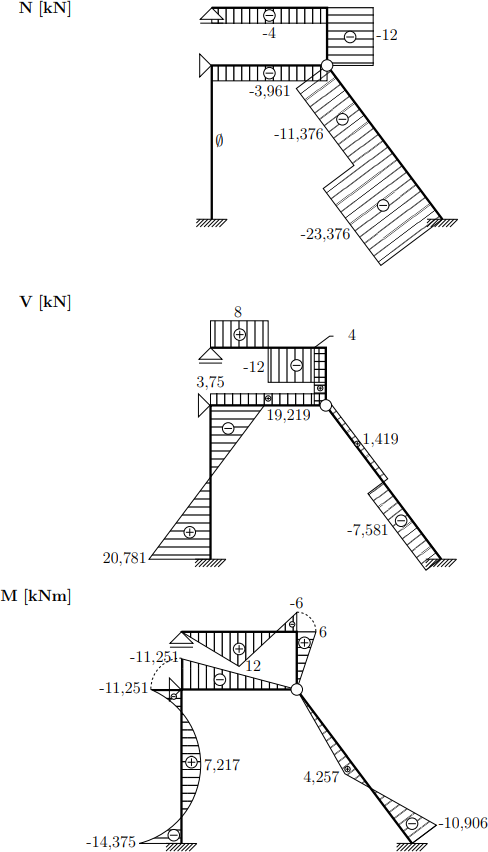
\includegraphics{assets/figures/framesss/example_internal_forces.png}
    \caption[Vnitřní síly na konstrukci]{Vnitřní síly na konstrukci, převzato z \cite[Příklad 5.2]{sbirka_prikladu}}
    \label{fig:framesss_example_internal_forces}
\end{figure}

\begin{table}[H]
    \setlength{\tabcolsep}{10pt}
    \renewcommand{\arraystretch}{1.2}
    \rowcolors{2}{ctulightblue!20}{white}
    \begin{tabular}{ccrrr}
        \rowcolor{ctulightblue} \bfseries veličina & \bfseries rozměr & \bfseries LC1 & \bfseries CO1 & \bfseries Sbírka \\ 
            $R_{1,\gls{x}}$ & $\SI{}{\kilo\newton}$ & -20.781 & -20.781 & -20.781 \\
            $R_{1,\gls{z}}$ & $\SI{}{\kilo\newton}$ &   0.000 &   0.000 &   0.000 \\
            \rowcolor{yellow!15}$M_{1,\gls{y}}$ & $\SI{}{\kilo\newton\metre}$ & -14.375 & -14.375 &  14.375 \\
            $R_{2,\gls{x}}$ & $\SI{}{\kilo\newton}$ & -15.258 & -15.258 & -15.258 \\
            \rowcolor{yellow!15}$R_{2,\gls{z}}$ & $\SI{}{\kilo\newton}$ &   3.750 &   3.750 &   -3.750 \\
            $R_{4,\gls{x}}$ & $\SI{}{\kilo\newton}$ &  -7.961 &  -7.961 &  -7.961 \\
            \rowcolor{yellow!15}$R_{4,\gls{z}}$ & $\SI{}{\kilo\newton}$ &  23.250 &  23.250 &  -23.249 \\
            \rowcolor{yellow!15}$M_{4,\gls{y}}$ & $\SI{}{\kilo\newton}$ &  10.905 &  10.905 &  -10.906 \\
            \rowcolor{yellow!15}$R_{6,\gls{z}}$ & $\SI{}{\kilo\newton}$ &   8.000 &   8.000 &  -8.000 \\
            $\gls{phi_i}[2]$ & $\SI{}{\radian}\cdot 10^{-5}$ & -6.942 & -6.942 & 6.942 \\
            \rowcolor{red!8}$\gls{u_i}[3]$ & $\SI{}{\metre}\cdot 10^{-5}$ & -9.902 & -9.902 & -9.903 \\
            \rowcolor{yellow!15}$\gls{w_i}[3]$ & $\SI{}{\metre}\cdot 10^{-4}$ & -9.168 & -9.168 & 9.168 \\
            $\gls{axial_force}_{1,2}$ & $\SI{}{\kilo\newton}$ & 0.000 & 0.000 & 0.000 \\
            %
            $\gls{axial_force}_{2,3}$ & $\SI{}{\kilo\newton}$ & -3.961 & -3.961 & -3.961 \\
            %
            $\min(\gls{axial_force}_{3,4})$ & $\SI{}{\kilo\newton}$ & -23.376 & -23.376 & -23.376 \\
            $\max(\gls{axial_force}_{3,4})$ & $\SI{}{\kilo\newton}$ & -11.376 & -11.376 & -11.376 \\
            %
            $\gls{axial_force}_{3,5}$ & $\SI{}{\kilo\newton}$ & -12.000 & -12.000 & -12.000 \\
            %
            $\gls{axial_force}_{6,5}$ & $\SI{}{\kilo\newton}$ & -4.000 & -4.000 & -4.000 \\
            %%%%%%%%%%%%%%%%%%%%%%%%%%%%%%%%%%%%%%%%%%%%%%%%%%%%%%%%%%%%%%%%%%%%%%%%%%%%%%%%%%%%%%%%%%
            $\min(\gls{shear_force}_{1,2})$ & $\SI{}{\kilo\newton}$ & -19.219 & -19.219 & -19.219 \\
            $\max(\gls{shear_force}_{1,2})$ & $\SI{}{\kilo\newton}$ & 20.781 & 20.781 & 20.781 \\
            %
            $\gls{shear_force}_{2,3}$ & $\SI{}{\kilo\newton}$ & 3.750 & 3.750 & 3.750 \\
            %
            $\min(\gls{shear_force}_{3,4})$ & $\SI{}{\kilo\newton}$ & -7.581 & -7.581 & -7.581 \\
            $\max(\gls{shear_force}_{3,4})$ & $\SI{}{\kilo\newton}$ & 1.419 & 1.419 & 1.419 \\
            %
            $\gls{shear_force}_{3,5}$ & $\SI{}{\kilo\newton}$ & 4.000 & 4.000 & 4.000 \\
            %
            $\min(\gls{shear_force}_{6,5})$ & $\SI{}{\kilo\newton}$ & -12.000 & -12.000 & -12.000 \\
            $\max(\gls{shear_force}_{6,5})$ & $\SI{}{\kilo\newton}$ & 8.000 & 8.000 & 8.000 \\
            %%%%%%%%%%%%%%%%%%%%%%%%%%%%%%%%%%%%%%%%%%%%%%%%%%%%%%%%%%%%%%%%%%%%%%%%%%%%%%%%%%%%%%%%%%
            $\min(\gls{bending_moment}_{1,2})$ & $\SI{}{\kilo\newton\meter}$ & -14.375 & -14.375 & -14.375 \\
            \rowcolor{red!8}$\max(\gls{bending_moment}_{1,2})$ & $\SI{}{\kilo\newton\meter}$ & 7.218 & 7.218 & 7.217 \\
            %
            $\min(\gls{bending_moment}_{2,3})$ & $\SI{}{\kilo\newton\meter}$ & -11.251 & -11.251 & -11.251 \\
            $\max(\gls{bending_moment}_{2,3})$ & $\SI{}{\kilo\newton\meter}$ & 0.000 & 0.000 & 0.000 \\
            %
            \rowcolor{red!8}$\min(\gls{bending_moment}_{3,4})$ & $\SI{}{\kilo\newton\meter}$ & -10.905 & -10.905 & -10.906 \\
            $\max(\gls{bending_moment}_{3,4})$ & $\SI{}{\kilo\newton\meter}$ & 4.257 & 4.257 & 4.257 \\
            %
            $\min(\gls{bending_moment}_{3,5})$ & $\SI{}{\kilo\newton\meter}$ & 0.000 & 0.000 & 0.000 \\
            $\max(\gls{bending_moment}_{3,5})$ & $\SI{}{\kilo\newton\meter}$ & 6.000 & 6.000 & 6.000 \\
            %
            $\min(\gls{bending_moment}_{6,5})$ & $\SI{}{\kilo\newton\meter}$ & -6.000 & -6.000 & -6.000 \\
            $\max(\gls{bending_moment}_{6,5})$ & $\SI{}{\kilo\newton\meter}$ & 12.000 & 12.000 & 12.000 
    \end{tabular}
    \caption{Porovnání výsledků}
    \label{tab:example_values}
\end{table}

V \autoref{tab:example_values} jsou uvedeny hodnoty vypočítané knihovnou \texttt{framesss} a srovnány s referenčními hodnotami ze \textit{Sbírky příkladů stavební mechaniky} \cite{sbirka_prikladu}. Testování probíhalo ve dvou různých scénářích: zatěžovací stav (LC1) a kombinace zatěžovacích stavů (CO1). LC1 představuje stav, kde je veškeré zatížení aplikováno najednou. CO1 je kombinace jednotlivých zatěžovacích stavů, kde každé zatížení bylo odděleně definováno a hodnota zatížení byla vydělena předem definovaným součinitel. Následně byly tyto zatěžovací stavy zkombinovány do kombinace zatěžovacích stavů s těmito součiniteli.

Porovnání výsledků ukazuje, že hodnoty vypočítané knihovnou \texttt{framesss} jsou téměř stejné jako referenční hodnoty, přičemž rozdíly (vyznačené \colorbox{red!8}{červenou barvou}) se nacházejí v rámci zaokrouhlovací chyby.

Hodnoty posunutí a reakcí ve směru osy \gls{Z} a hodnoty pootočení a momentů okolo osy \gls{Y} vykazují opačné znaménko (vyznačeno \colorbox{yellow!15}{žlutou barvou}) ve srovnání s referenčními hodnotami, což je způsobeno rozdílným natočením globálního souřadného systému, viz obr. \ref{fig:example_coordinate_systems}. Systém ze sbírky je vlevo, uvažovaný systém při zadávání konstrukce v této práci vpravo. Při stanovení kladného směru pootočení platí pravidlo pravé ruky.

\begin{figure}[H]
    \begin{tikzpicture}[>={Stealth[inset=0pt,length=8pt,angle'=28,round]}]
    \draw[->] (0, 0) -- ++(2,0) node[above right=0 and -1] {$+\gls{X}$, $+\gls{u_i}$, $+R_{\gls{x},i}$};
    \draw[->] (0, 0) -- ++(0,-2) node[right] {$+\gls{Z}$, $+\gls{w_i}$, $+R_{\gls{z},i}$};
    \draw[->,domain=180:450] plot ({cos(\x)}, {sin(\x)}) node[above] {$+\gls{phi_i}$, $+R_{M,\gls{y},i}$};

    \draw[->] (6, 0) -- ++(2,0) node[above right=0 and -1] {$+\gls{X}$, $+\gls{u_i}$, $+R_{\gls{x},i}$};
    \draw[->] (6, 0) -- ++(0,2) node[right] {$+\gls{Z}$, $+\gls{w_i}$, $+R_{\gls{z},i}$};
    \draw[->,domain=180:-90] plot ({6+cos(\x)}, {sin(\x)}) node[below] {$+\gls{phi_i}$, $+R_{M,\gls{y},i}$};
\end{tikzpicture}
    \caption{Porovnání souřadných systémů}
    \label{fig:example_coordinate_systems}
\end{figure}

